% Supporting Information for Analytical Chemistry.
% Built by paper/build_si.ps1; numbers come from values.tex, which is written
% by run/05_paper_assets.py, so nothing here is typed by hand either.
\documentclass[journal=ancham,manuscript=suppinfo]{achemso}

\usepackage[T1]{fontenc}
\usepackage{mathptmx}
\usepackage[utf8]{inputenc}
\usepackage{amsmath,amssymb}
\usepackage{graphicx}
\usepackage{url}
\usepackage{booktabs}
\usepackage{siunitx}
\usepackage{longtable}
\graphicspath{{figures/}}

\IfFileExists{values.tex}{% auto-generated by run/05_paper_assets.py -- do not edit
\newcommand{\Nacq}{108}
\newcommand{\Nfittable}{40}
\newcommand{\Nrawmap}{23}
\newcommand{\Nrawmaptext}{1}
\newcommand{\Nrawscan}{2}
\newcommand{\Nspecimen}{3}
\newcommand{\Nconfig}{16}
\newcommand{\Nskipped}{164}
\newcommand{\Nlsix}{57}
\newcommand{\Nlsixfail}{563}
\newcommand{\Ndupgroups}{5}
\newcommand{\KGnodes}{236}
\newcommand{\KGedges}{636}
\newcommand{\KGcommunities}{23}
\newcommand{\KGmodularity}{0.65}
\newcommand{\KGpurity}{0.86}
\newcommand{\SplatN}{2904}
\newcommand{\SplatParams}{31944}
\newcommand{\SplatPSNRtrain}{27.4}
\newcommand{\SplatPSNReval}{25.0}
\newcommand{\SplatSSIM}{0.956}
\newcommand{\SplatSAM}{0.224}
\newcommand{\SplatCompression}{37.7}
\newcommand{\SplatCompressionBinned}{9.4}
\newcommand{\SplatAniso}{1.84}
\newcommand{\SplatAmpBands}{77.7}
\newcommand{\SplatBandSpan}{28.0}
\newcommand{\SplatSeconds}{244}
\newcommand{\SplatRawValues}{1203040}
\newcommand{\SplatAcq}{acq-0059}
\newcommand{\SplatMapNx}{81}
\newcommand{\SplatMapNy}{91}
\newcommand{\SplatMapK}{292}
\newcommand{\SplatMaskPts}{4120}
\newcommand{\SplatNfits}{6}
\newcommand{\SplatResidNoise}{0.84}
\newcommand{\SplatResidNoiseMin}{0.70}
\newcommand{\SplatResidNoiseMax}{1.34}
\newcommand{\SplatRhoMin}{12}
\newcommand{\SplatRhoMax}{56}
\newcommand{\SplatComprMin}{8.1}
\newcommand{\SplatComprMax}{37.7}
\newcommand{\SplatPSNRevalMin}{17.9}
\newcommand{\SplatPSNRevalMax}{27.2}
\newcommand{\Nrawmapfit}{6}
\newcommand{\MLDenoiseN}{1200}
\newcommand{\MLDenoiseMap}{acq-0057}
\newcommand{\MLRefFilter}{SG(2,5)}
\newcommand{\MLSplatRho}{8}
\newcommand{\MLSplatN}{3806}
\newcommand{\MLNoiseMult}{1.5}
\newcommand{\MLBestDenoiser}{PCA (rank 217)}
\newcommand{\MLDenoiseGain}{1.16}
\newcommand{\MLNmodels}{30}
\newcommand{\MLParticleAcc}{81.04}
\newcommand{\MLParticleModel}{NearestCentroid}
\newcommand{\MLParticleTrainMaps}{14}
\newcommand{\MLParticleTestMaps}{6}
\newcommand{\MLParticleClasses}{2}
\newcommand{\MLParticleBase}{63.00}
\newcommand{\MLParticleBeat}{26}
\newcommand{\MLParticleLift}{18.04}
\newcommand{\MLParticleClassesTested}{2}
\newcommand{\MLConfigAcc}{46.55}
\newcommand{\MLConfigModel}{ExtraTrees}
\newcommand{\MLConfigTrainMaps}{13}
\newcommand{\MLConfigTestMaps}{5}
\newcommand{\MLConfigClasses}{11}
\newcommand{\MLConfigBase}{21.18}
\newcommand{\MLConfigBeat}{28}
\newcommand{\MLConfigLift}{25.37}
\newcommand{\MLConfigClassesTested}{3}
\newcommand{\AblMin}{0.283}
\newcommand{\AblMax}{0.290}
\newcommand{\AblSpread}{2.4}
\newcommand{\AblNproto}{5}
\newcommand{\SplatFloorBand}{20}
\newcommand{\SplatNatFloor}{2}
\newcommand{\SplatNnearFloor}{4}
\newcommand{\SplatPSNRSNRr}{0.83}
\newcommand{\SplatSNRmin}{3.8}
\newcommand{\SplatSNRmax}{13.1}
\newcommand{\AblNmaps}{8}
\newcommand{\AblSpreadMedian}{4.9}
\newcommand{\AblSpreadMax}{14.8}
\newcommand{\AblSpreadRaw}{80.7}
}{}
\providecommand{\Nacq}{n/a}\providecommand{\Nrawmap}{n/a}
\providecommand{\Nrawmaptext}{n/a}\providecommand{\Nspecimen}{n/a}
\providecommand{\Nconfig}{n/a}\providecommand{\Nlsix}{n/a}
\providecommand{\Nlsixfail}{n/a}\providecommand{\Ndupgroups}{n/a}
\providecommand{\SplatNfits}{n/a}\providecommand{\SplatAcq}{n/a}
\providecommand{\MLNmodels}{n/a}\providecommand{\MLDenoiseMap}{n/a}
\providecommand{\MLDenoiseN}{n/a}\providecommand{\MLRefFilter}{n/a}
\providecommand{\KGnodes}{n/a}\providecommand{\KGedges}{n/a}
\providecommand{\KGcommunities}{n/a}\providecommand{\KGmodularity}{n/a}
\providecommand{\AblNmaps}{n/a}\providecommand{\AblNproto}{n/a}

\newcommand{\ramansp}{\textsc{ramansp}}
\newcommand{\code}[1]{\texttt{\small #1}}

\author{Siddhartha Pahari}
\affiliation{Department of Chemical Engineering \& Applied Chemistry,
University of Toronto, 200 College Street, Toronto, ON M5S 3E5, Canada}
\email{siddhartha.pahari@mail.utoronto.ca}

\author{Jainish Shailesh Solanki}
\affiliation{Leslie Dan Faculty of Pharmacy, University of Toronto,
144 College Street, Toronto, ON M5S 3M2, Canada}
\alsoaffiliation{Department of Mechanical and Industrial Engineering, University of
Toronto, 5 King's College Road, Toronto, ON M5S 3G8, Canada}
\email{jainish.solanki@utoronto.ca}

\title{Supporting Information:
Reading the whole corpus: a reproducible cross-sample Raman workflow for
materials characterisation, with a spectral 3D Gaussian splatting
representation for hyperspectral maps}

\begin{document}

\section{Contents}

This document contains the per-map reconstruction figures for every fitted
acquisition, the full model and denoiser benchmark tables, and the corpus and
knowledge-graph summary tables that the main text quotes selectively. Machine
readable versions of every table, the knowledge graph in GraphML, the fitted
fields and the anonymity-gate report are distributed with the released code
rather than reproduced here.

\paragraph{Code and companion site.}
The \ramansp{} package and the full pipeline are released at
\url{https://github.com/siddhartha18pahari/RAMANSP}. A companion site at
\url{https://ramansp.vercel.app} carries the same material in browsable form,
including an interactive view of the cross-sample knowledge graph, in which the
nodes and edges can be dragged, zoomed and inspected one at a time rather than
read off a static drawing, together with every figure at full resolution and all
three renderings of the manuscript.

\section{Corpus and anonymisation}

The corpus holds \Nacq{} acquisitions drawn from \Nspecimen{} specimen codes
and \Nconfig{} acquisition configurations. Of these, \Nlsix{} were decoded
directly from the vendor's binary container; \Nlsixfail{} files in an older
container variant are not yet handled and are listed in the release. Reading
the binaries takes the number of usable hyperspectral maps from
\Nrawmaptext{} to \Nrawmap. Byte-identical duplicate exports are detected by
content hash, and \Ndupgroups{} groups were found.

Every specimen identifier, material designation, person name and dated session
folder is replaced by an opaque code in a single pass, and the forward map is
written to a private file that is excluded from the release. A gate scans
everything shareable for surviving identifiers and fails the build on a hit.

\begin{table}[h]\centering
\caption{Composition of the anonymised corpus.}
\label{tab:si-corpus}
\IfFileExists{tables/corpus.tex}{\begin{tabular}{lr}
\toprule
acquisition kind & count \\
\midrule
fit table & 40 \\
spectrum & 36 \\
raw map & 23 \\
autocal & 7 \\
raw scan & 2 \\
\midrule
total & 108 \\
\bottomrule
\end{tabular}
}{(table not built)}
\end{table}

\section{Knowledge graph}

\begin{table}[h]\centering
\caption{Knowledge-graph summary. Communities are extracted by greedy
modularity maximisation over the content sub-graph only, so provenance edges,
which are true by construction, cannot manufacture structure.}
\label{tab:si-kg}
\IfFileExists{tables/kg.tex}{\begin{tabular}{lr}
\toprule
quantity & value \\
\midrule
nodes & 236 \\
edges & 636 \\
communities & 23 \\
modularity $Q$ & 0.65 \\
community purity vs.\ class & 0.86 \\
\bottomrule
\end{tabular}
}{(table not built)}
\end{table}

The graph holds \KGnodes{} nodes and \KGedges{} edges in \KGcommunities{}
communities at modularity $Q=\KGmodularity$. The per-acquisition community
assignment is released as \code{tables/kg\_communities.csv}, and the graph
itself as \code{graph/knowledge\_graph.graphml} with an interactive browser
view alongside it.

\section{Spectral 3D Gaussian splatting: all fitted maps}

\begin{table}[h]\centering
\caption{Reconstruction across all \SplatNfits{} fitted maps. $\rho$ is
primitives per 1000 fitted voxels, and $r/\sigma$ is the held-out residual
divided by that map's own second-difference noise estimate, so a value at or
below one means the field is no further from the data than the data is from
itself.}
\label{tab:si-splat}
\IfFileExists{tables/splat.tex}{\begin{tabular}{lrrrrr}
\toprule
map & $N$ & $\rho$ & compr. & PSNR (dB) & $r/\sigma$ \\
\midrule
map 0042 & 2912 & 12 & 38.0 & 22.5 & 1.06 \\
map 0039 & 2912 & 13 & 36.2 & 22.9 & 1.02 \\
map 0028 & 2912 & 13 & 34.5 & 16.9 & 1.12 \\
map 0059 & 2912 & 15 & 29.6 & 19.1 & 1.09 \\
map 0016 & 2912 & 24 & 19.1 & 10.9 & 1.43 \\
map 0055 & 1239 & 56 & 8.1 & 27.2 & 0.70 \\
\bottomrule
\end{tabular}
}{(table not built)}
\end{table}

Figures~\ref{fig:si-bands-first} onwards give the measured and reconstructed
band maps for each fitted acquisition, on a shared colour scale per band with
the residual beside them, and the corresponding ellipsoid statistics. The
flagship map \SplatAcq{} appears in the main text and is not repeated here.

\clearpage
\section{Per-map reconstruction figures}

\begin{figure}[h]\centering
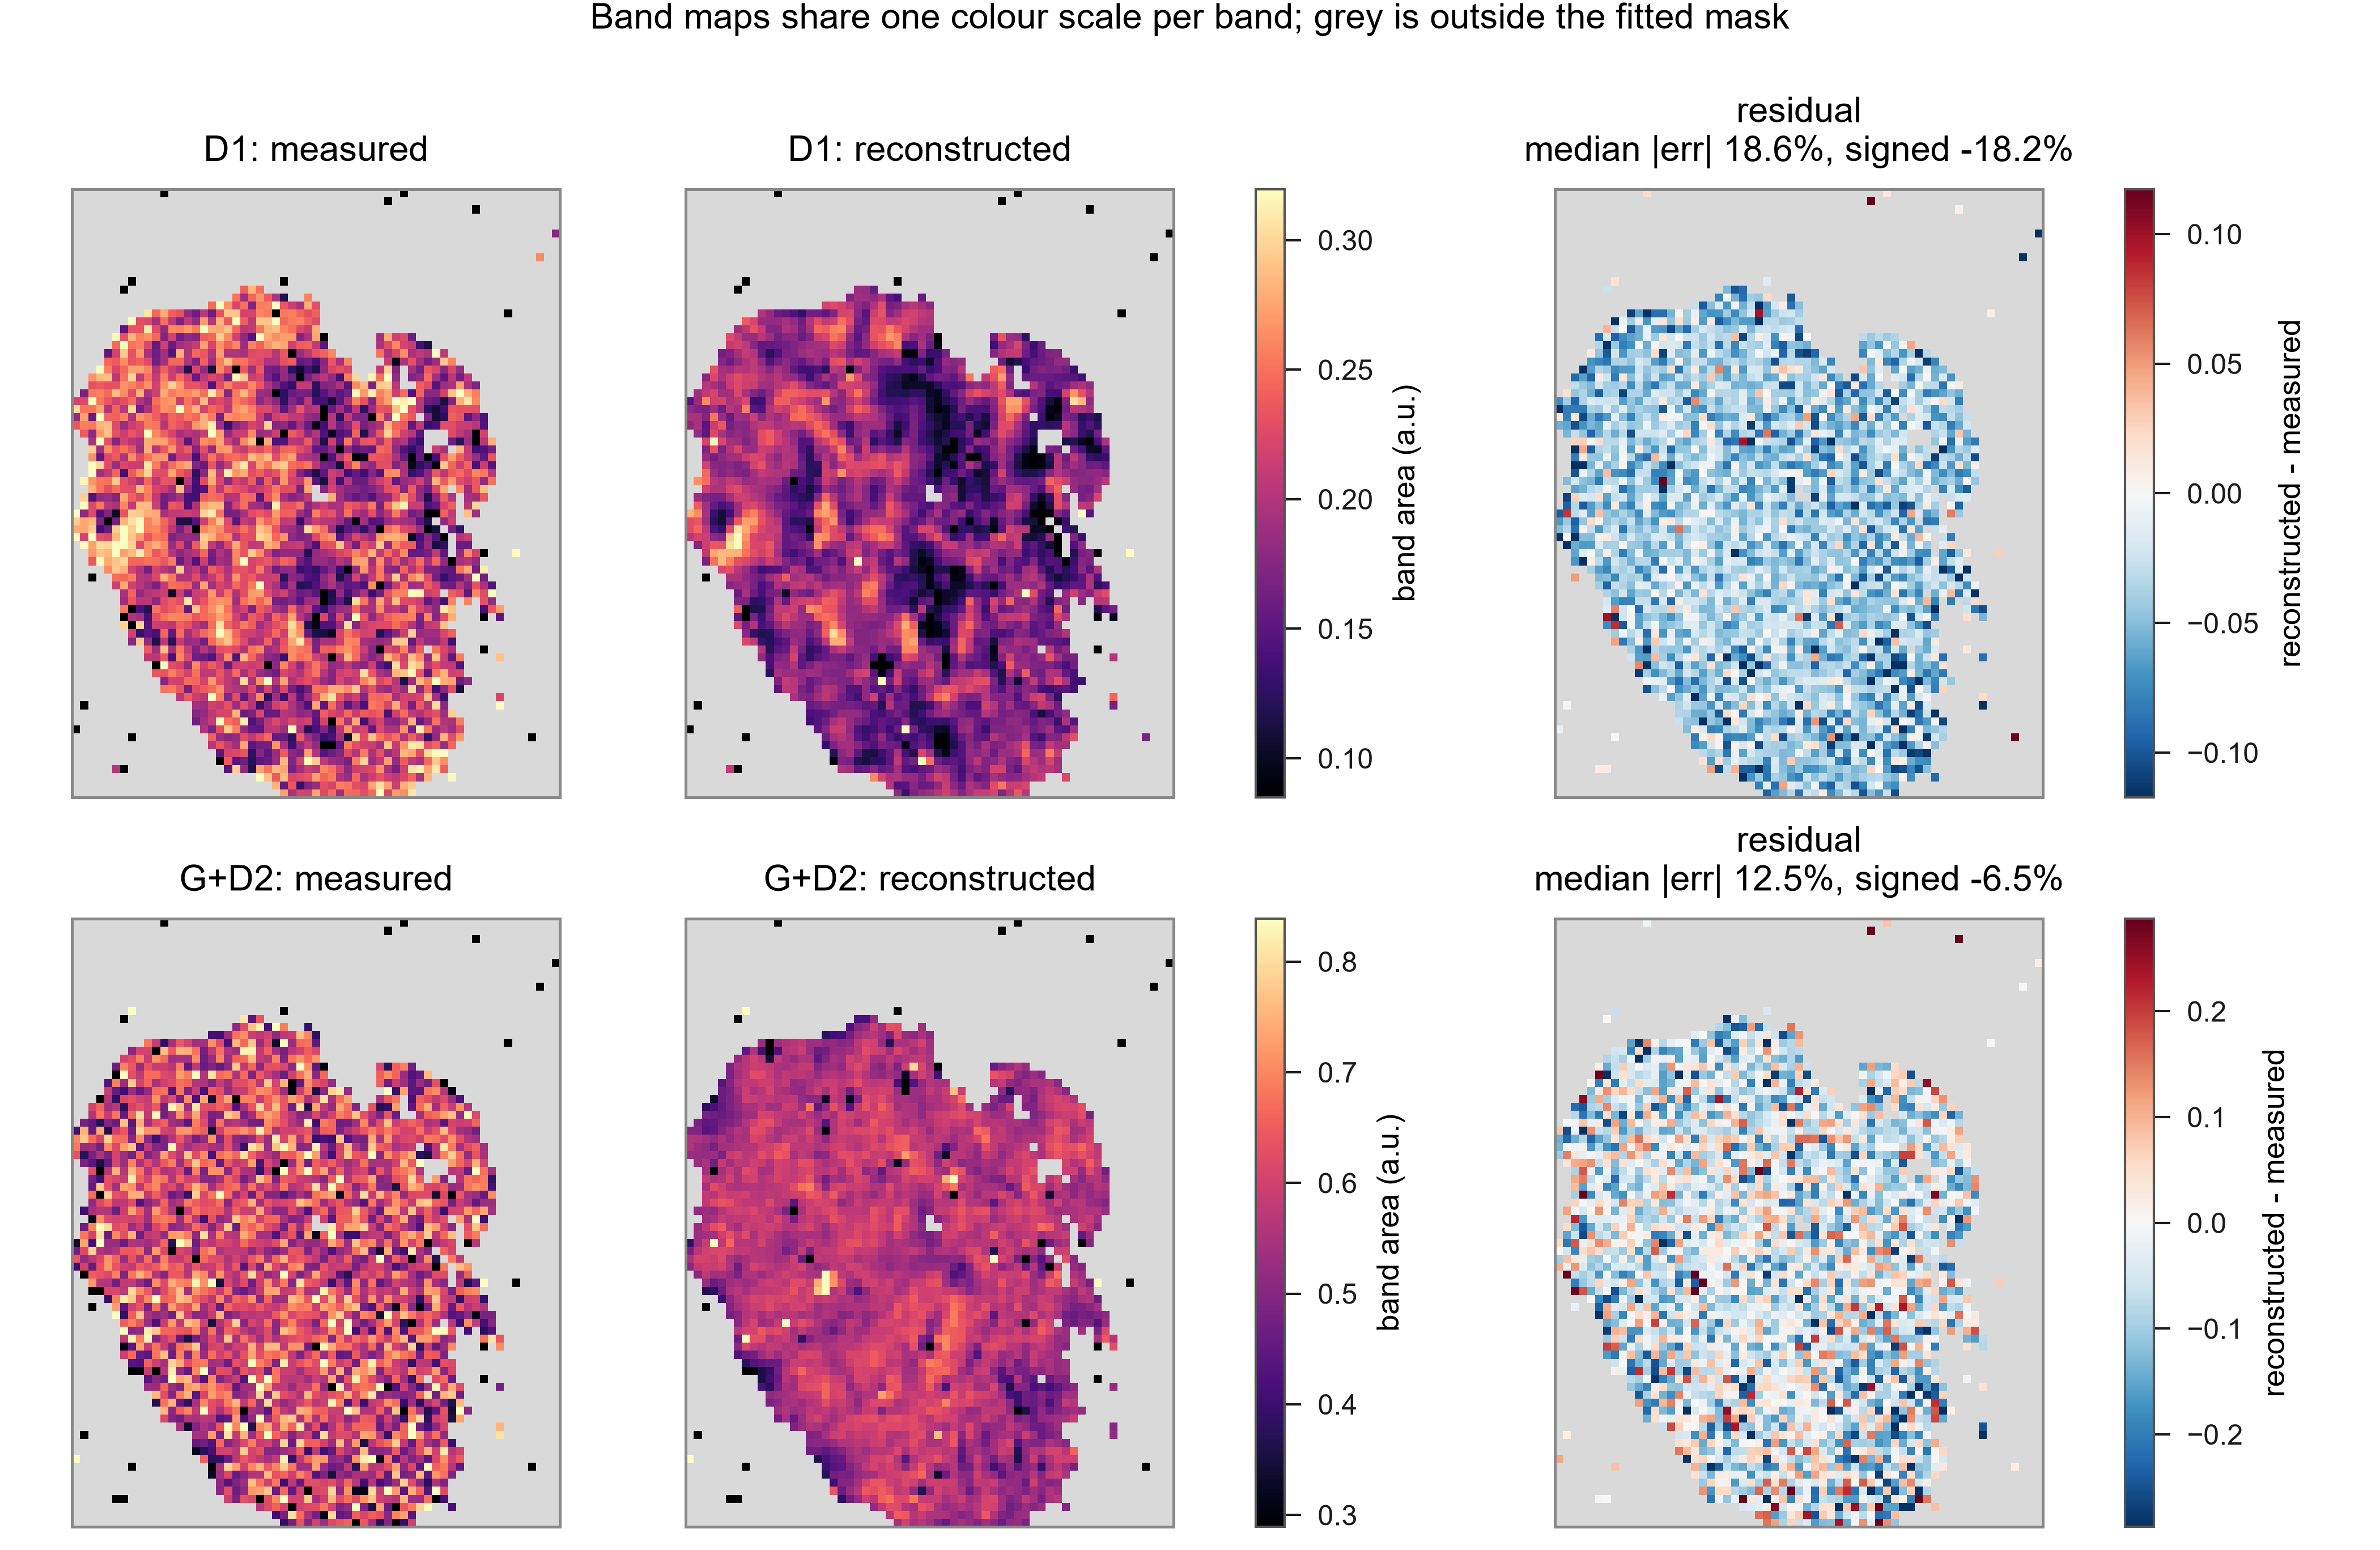
\includegraphics[width=\linewidth]{splat_acq-0016_bands}
\caption{Band maps for acq-0016: measured, reconstructed from the fitted field,
and residual, on a shared colour scale per band. Grey is outside the fitted
mask.}
\label{fig:si-bands-first}
\end{figure}

\begin{figure}[h]\centering
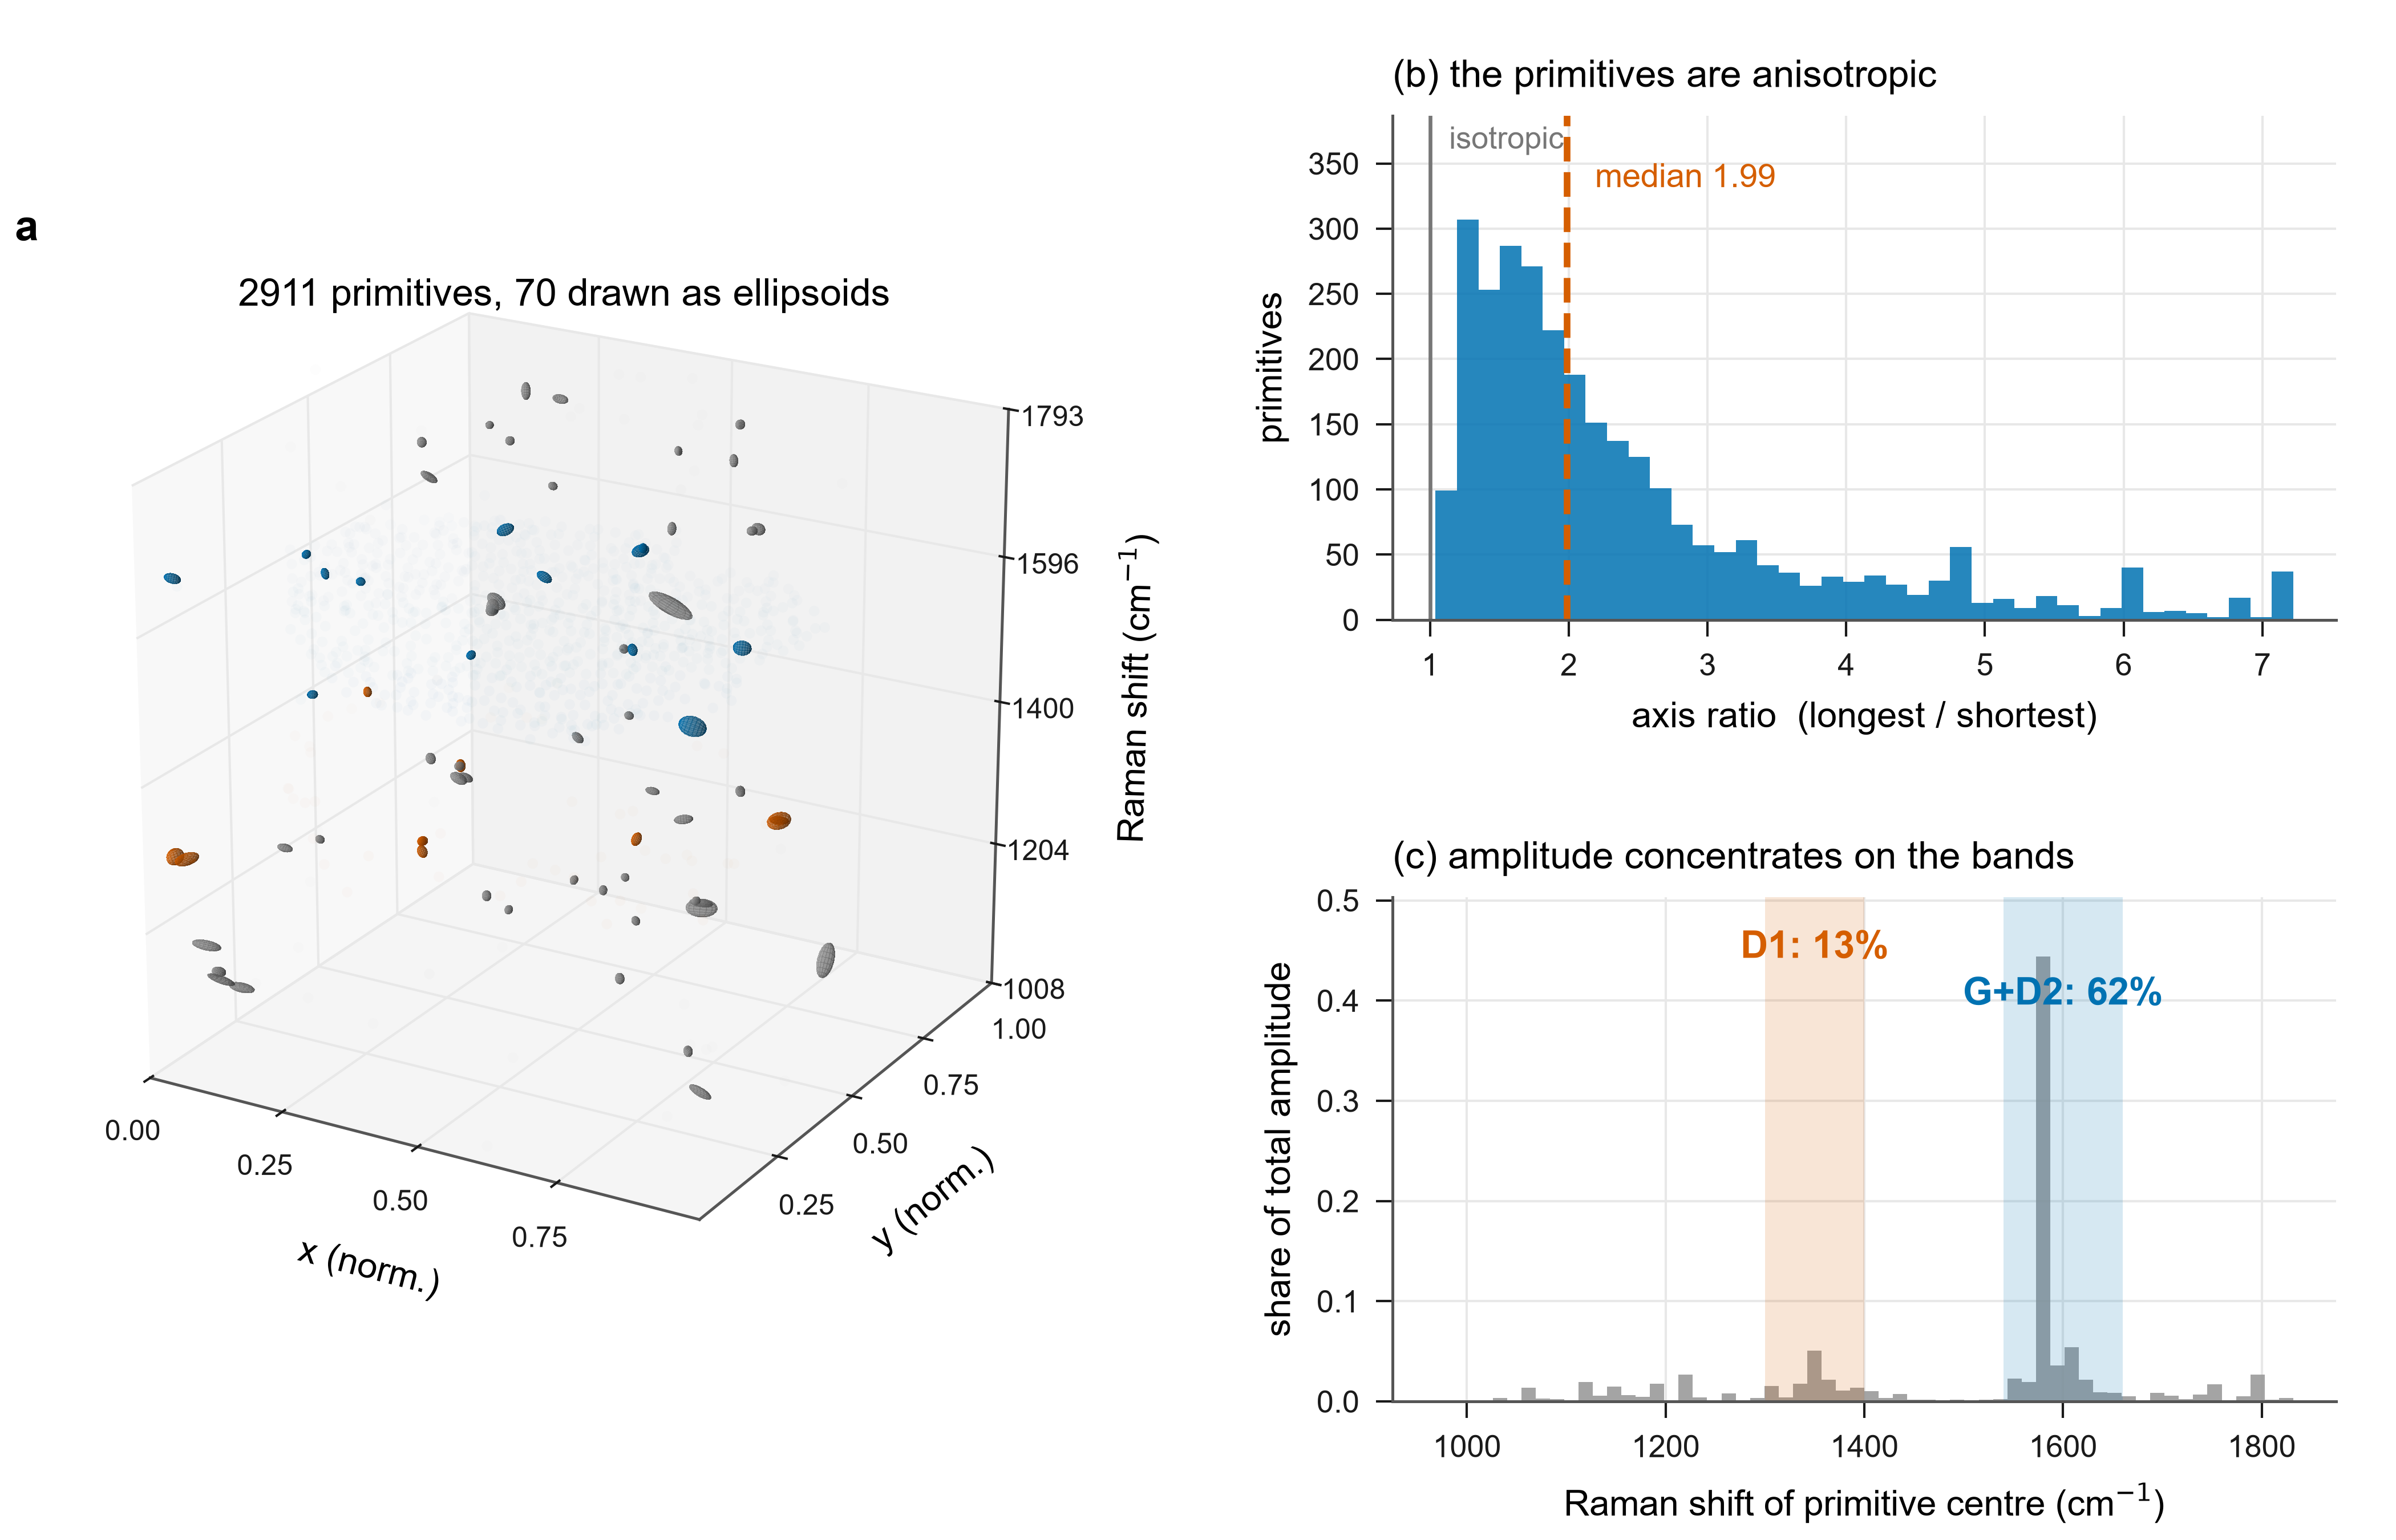
\includegraphics[width=\linewidth]{splat_acq-0016_ellipsoids}
\caption{Fitted primitives for acq-0016: the strongest drawn as ellipsoid
surfaces, the distribution of axis ratios, and the share of amplitude falling
inside each carbon band window.}
\end{figure}

\clearpage
\begin{figure}[h]\centering
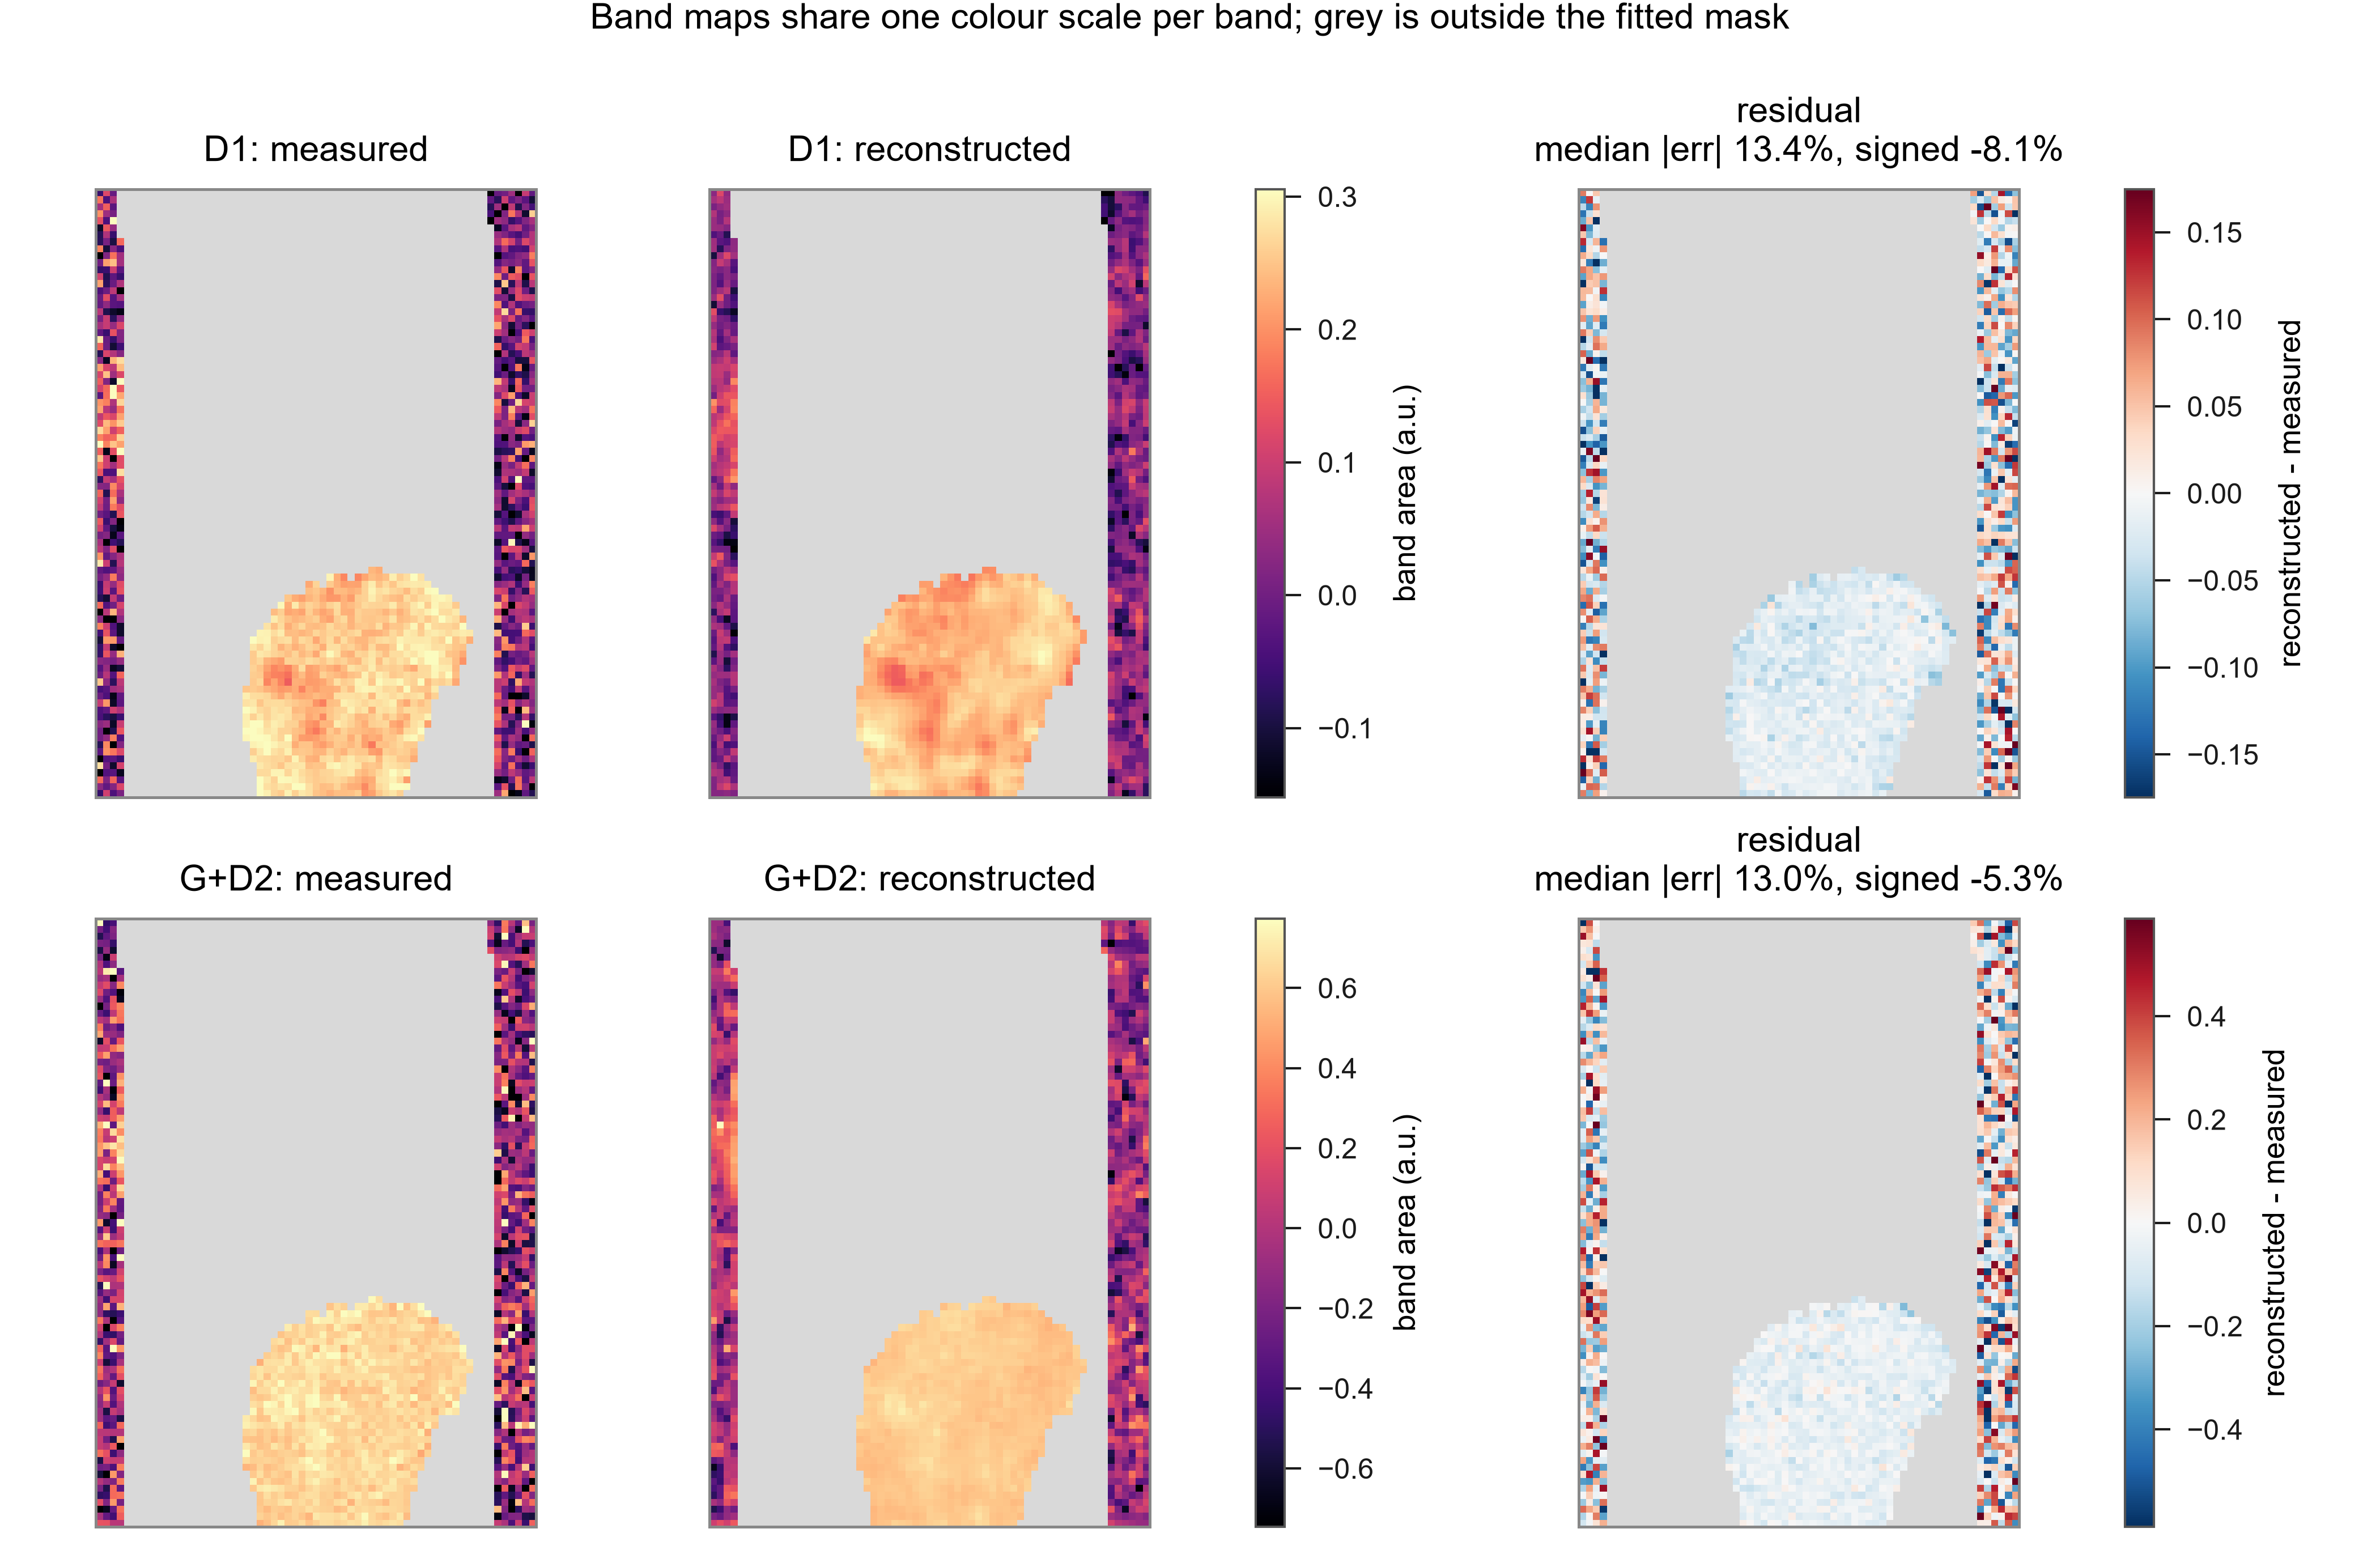
\includegraphics[width=\linewidth]{splat_acq-0028_bands}
\caption{Band maps for acq-0028, as Fig.~\ref{fig:si-bands-first}.}
\end{figure}

\begin{figure}[h]\centering
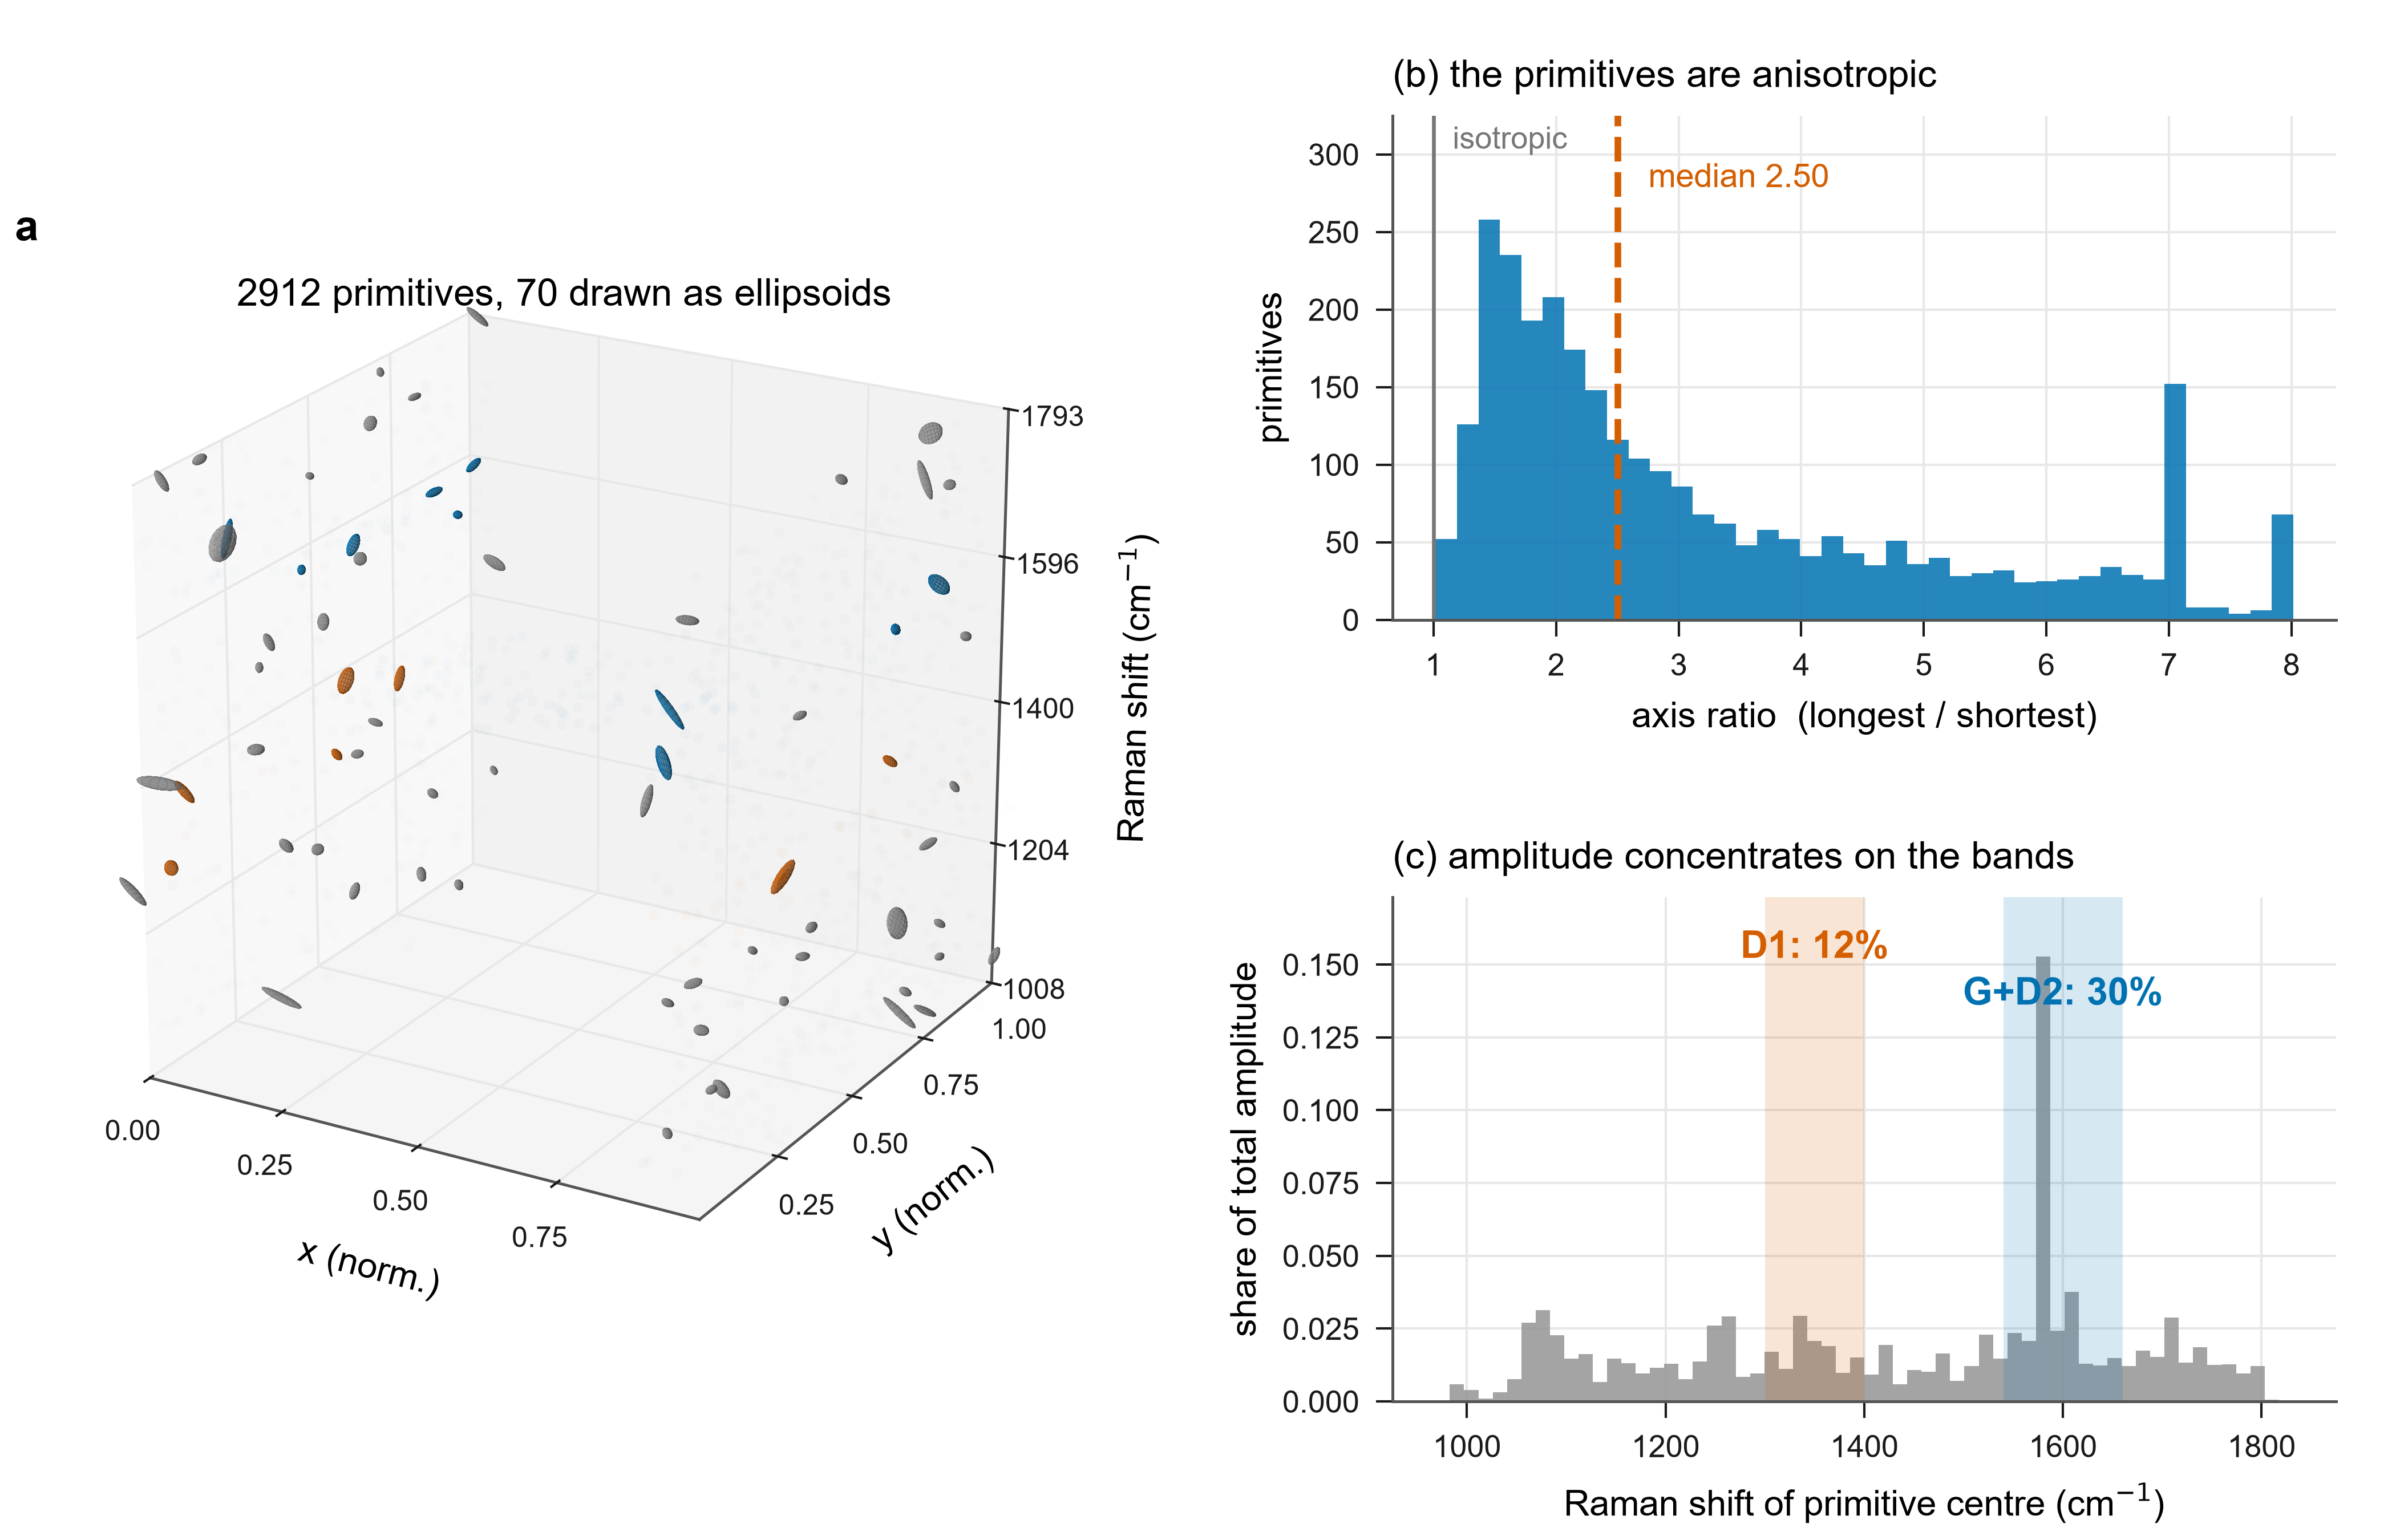
\includegraphics[width=\linewidth]{splat_acq-0028_ellipsoids}
\caption{Fitted primitives for acq-0028.}
\end{figure}

\clearpage
\begin{figure}[h]\centering
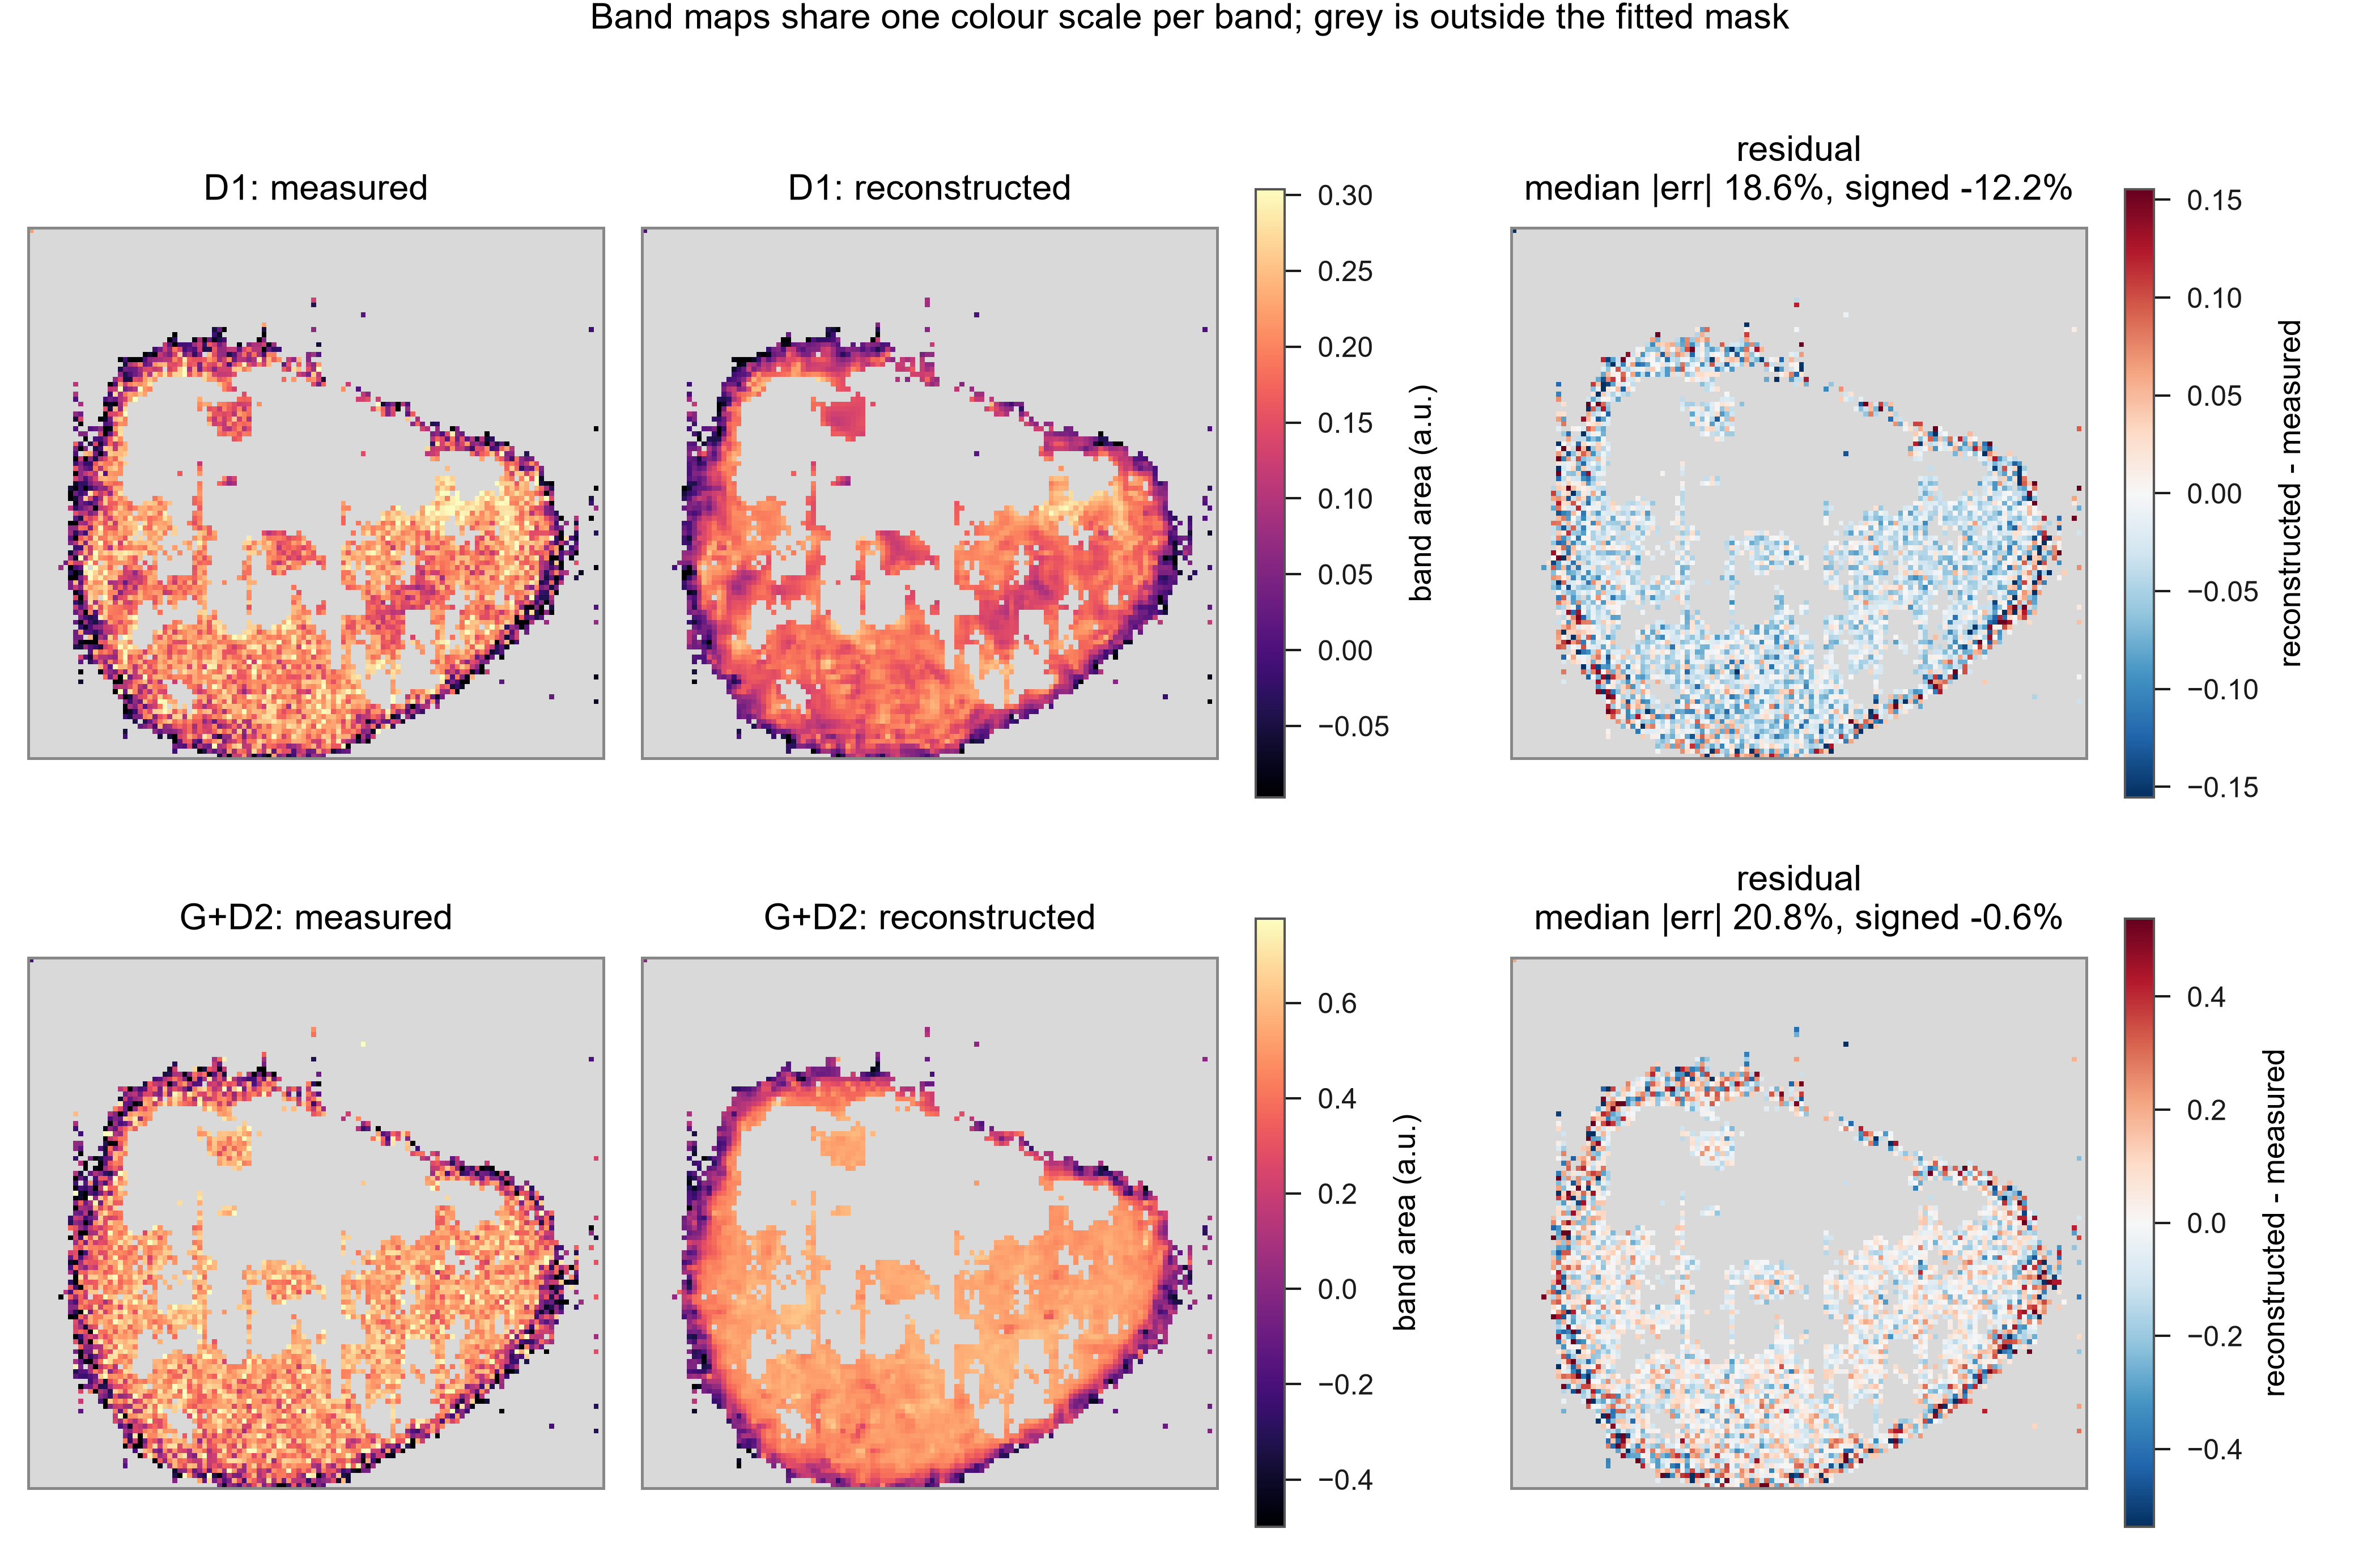
\includegraphics[width=\linewidth]{splat_acq-0039_bands}
\caption{Band maps for acq-0039, as Fig.~\ref{fig:si-bands-first}.}
\end{figure}

\begin{figure}[h]\centering
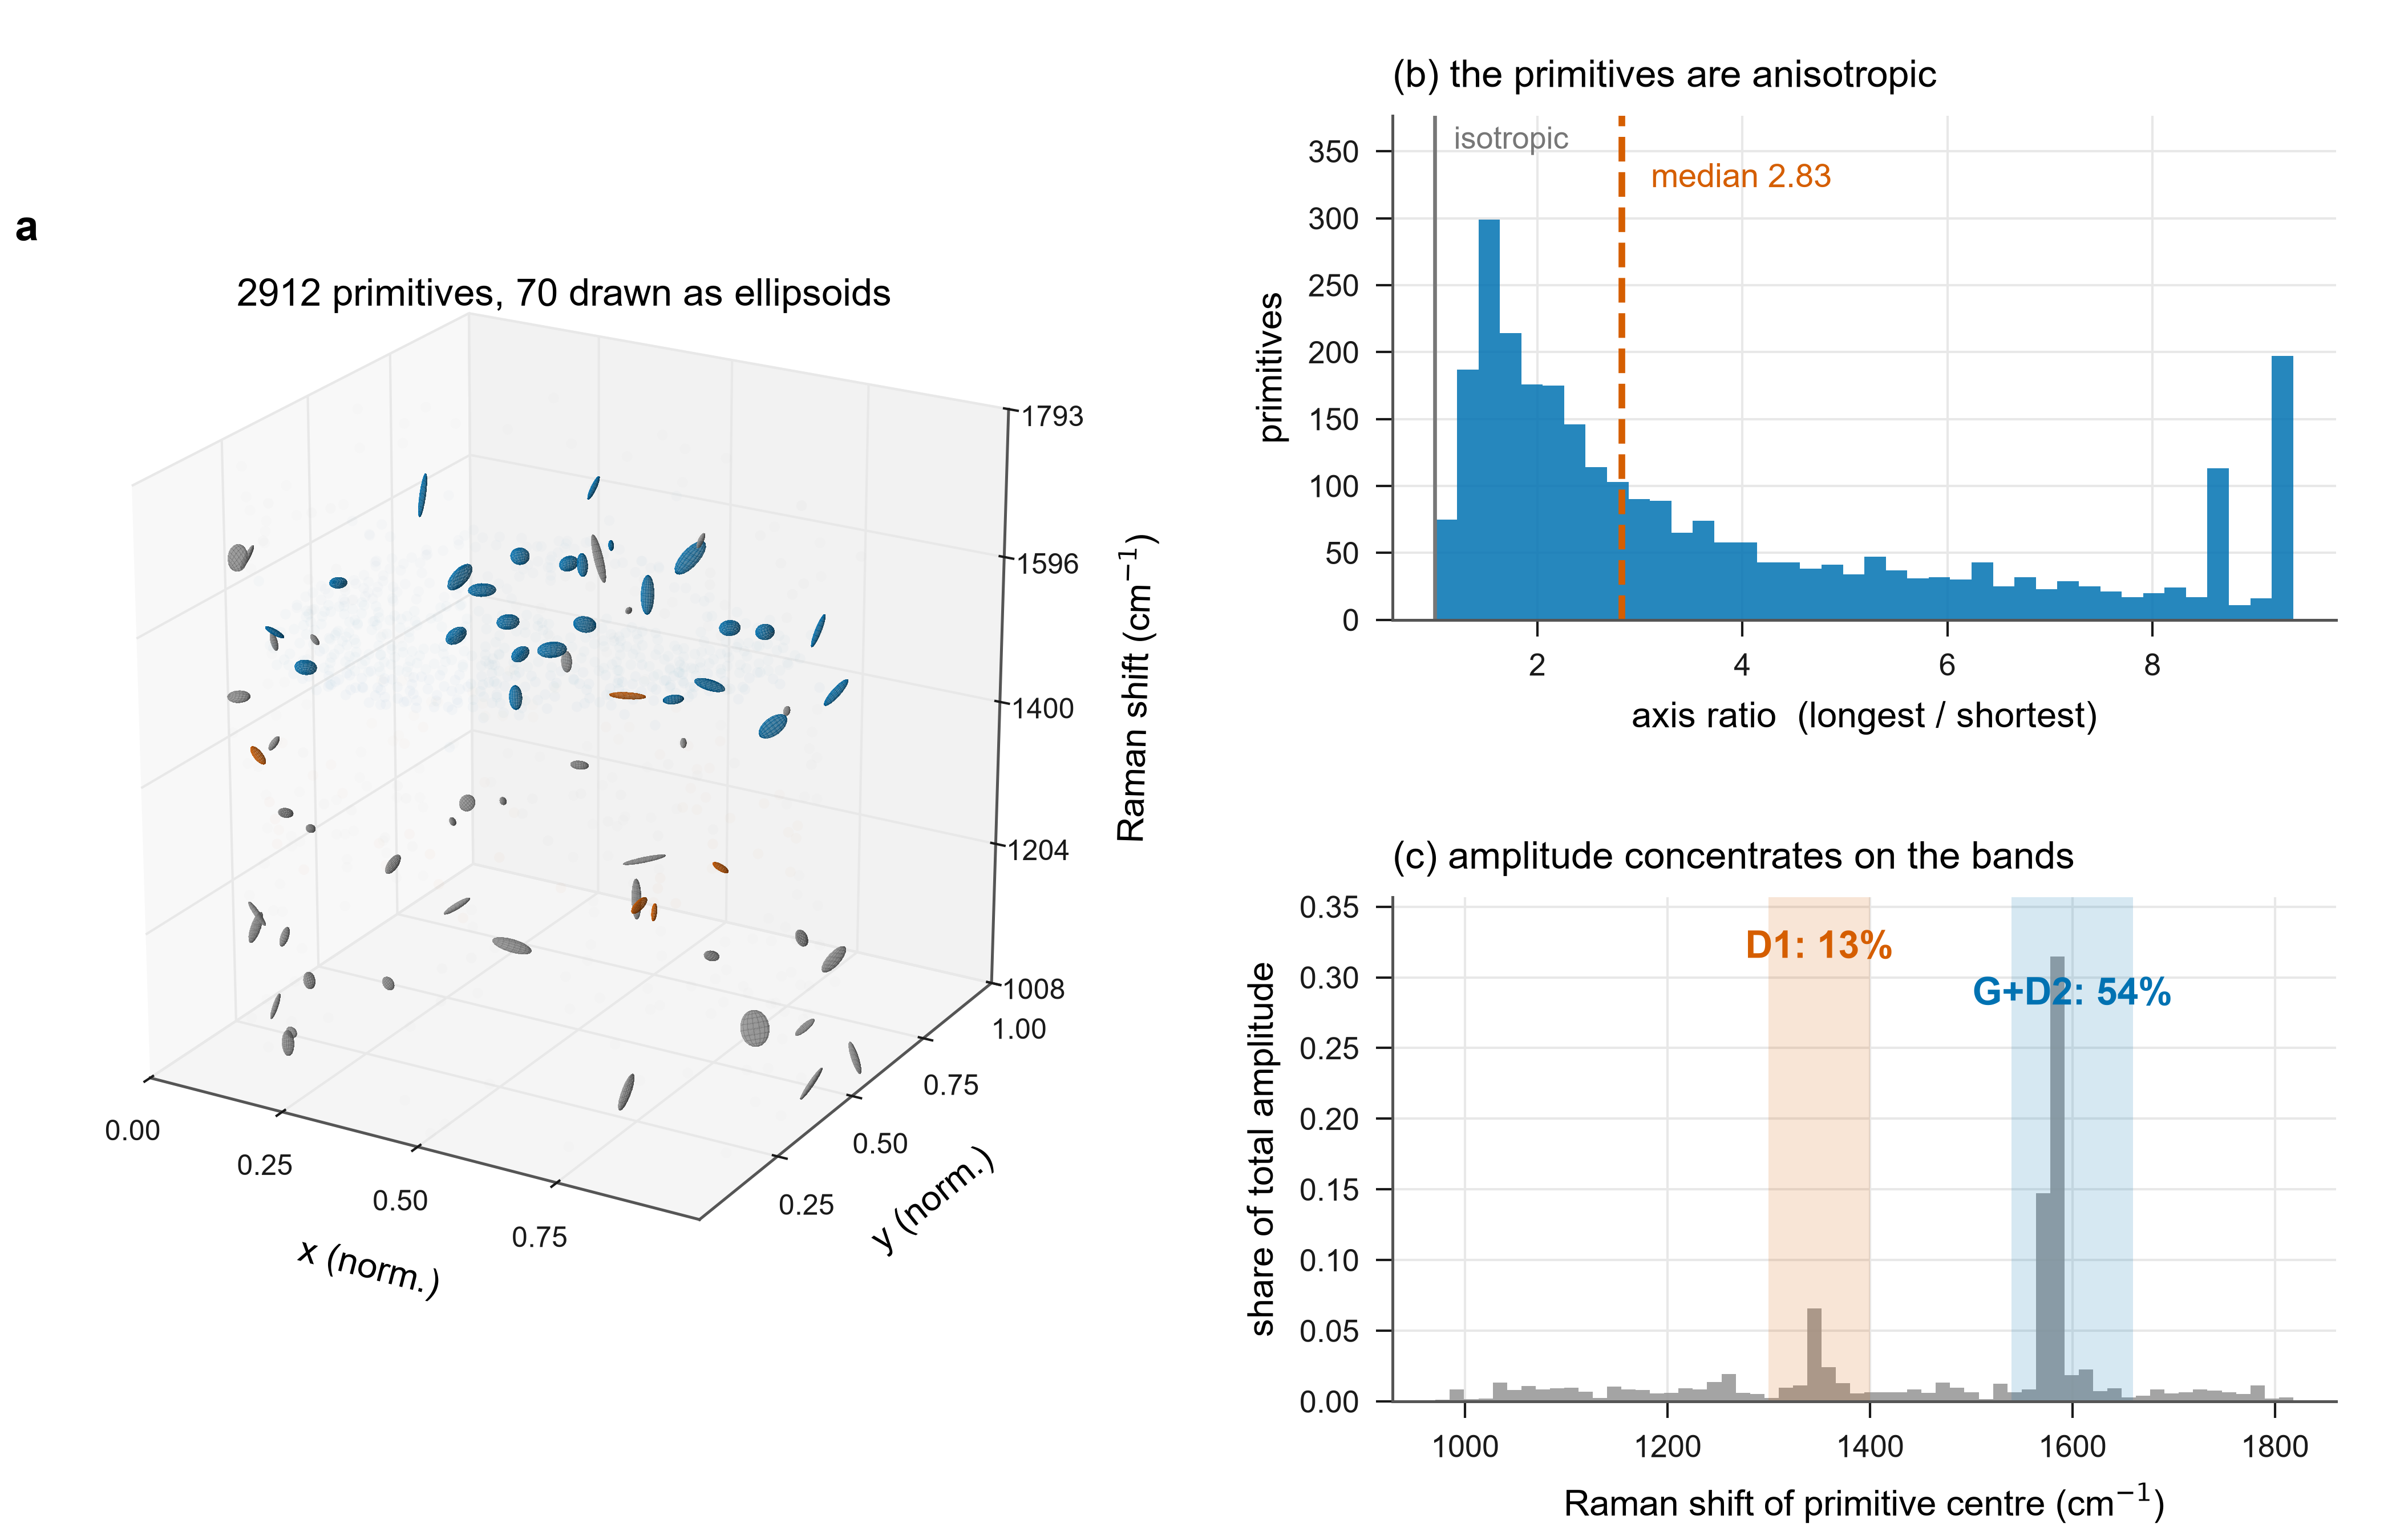
\includegraphics[width=\linewidth]{splat_acq-0039_ellipsoids}
\caption{Fitted primitives for acq-0039.}
\end{figure}

\clearpage
\begin{figure}[h]\centering
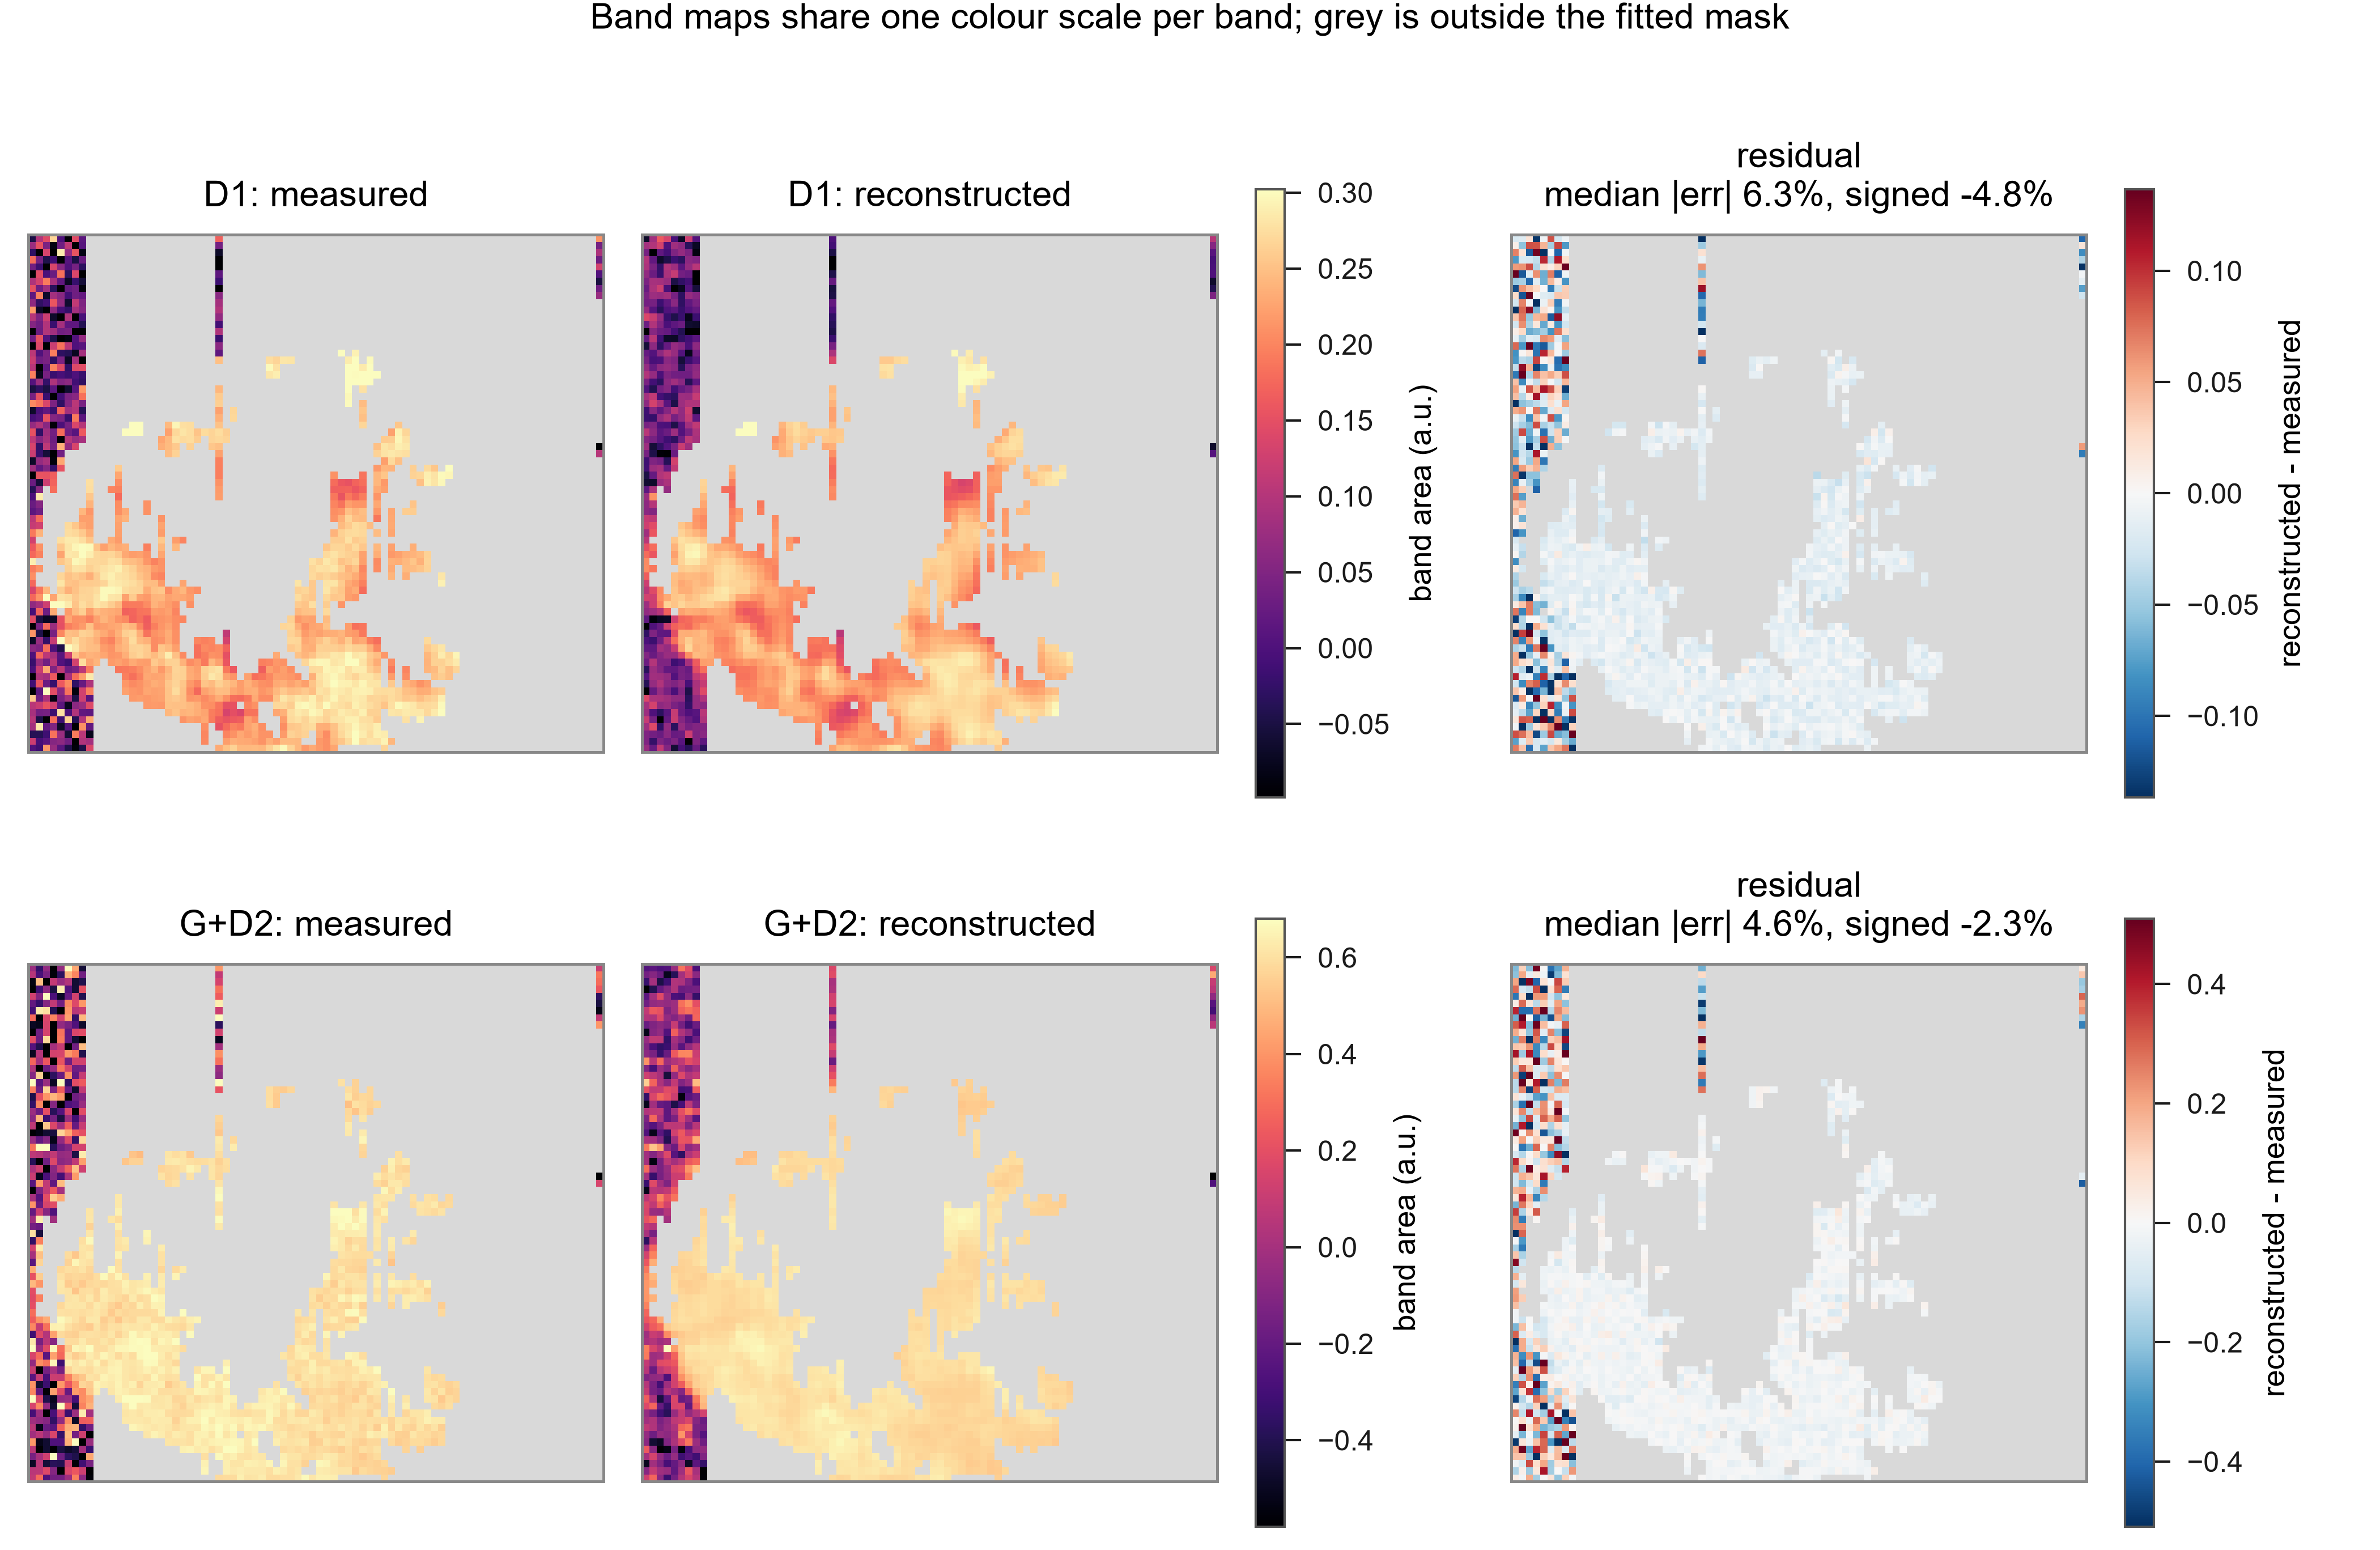
\includegraphics[width=\linewidth]{splat_acq-0042_bands}
\caption{Band maps for acq-0042, as Fig.~\ref{fig:si-bands-first}. This is one
of the maps on which the original particle mask was inverted; the figure shown
is from the corrected mask.}
\end{figure}

\begin{figure}[h]\centering
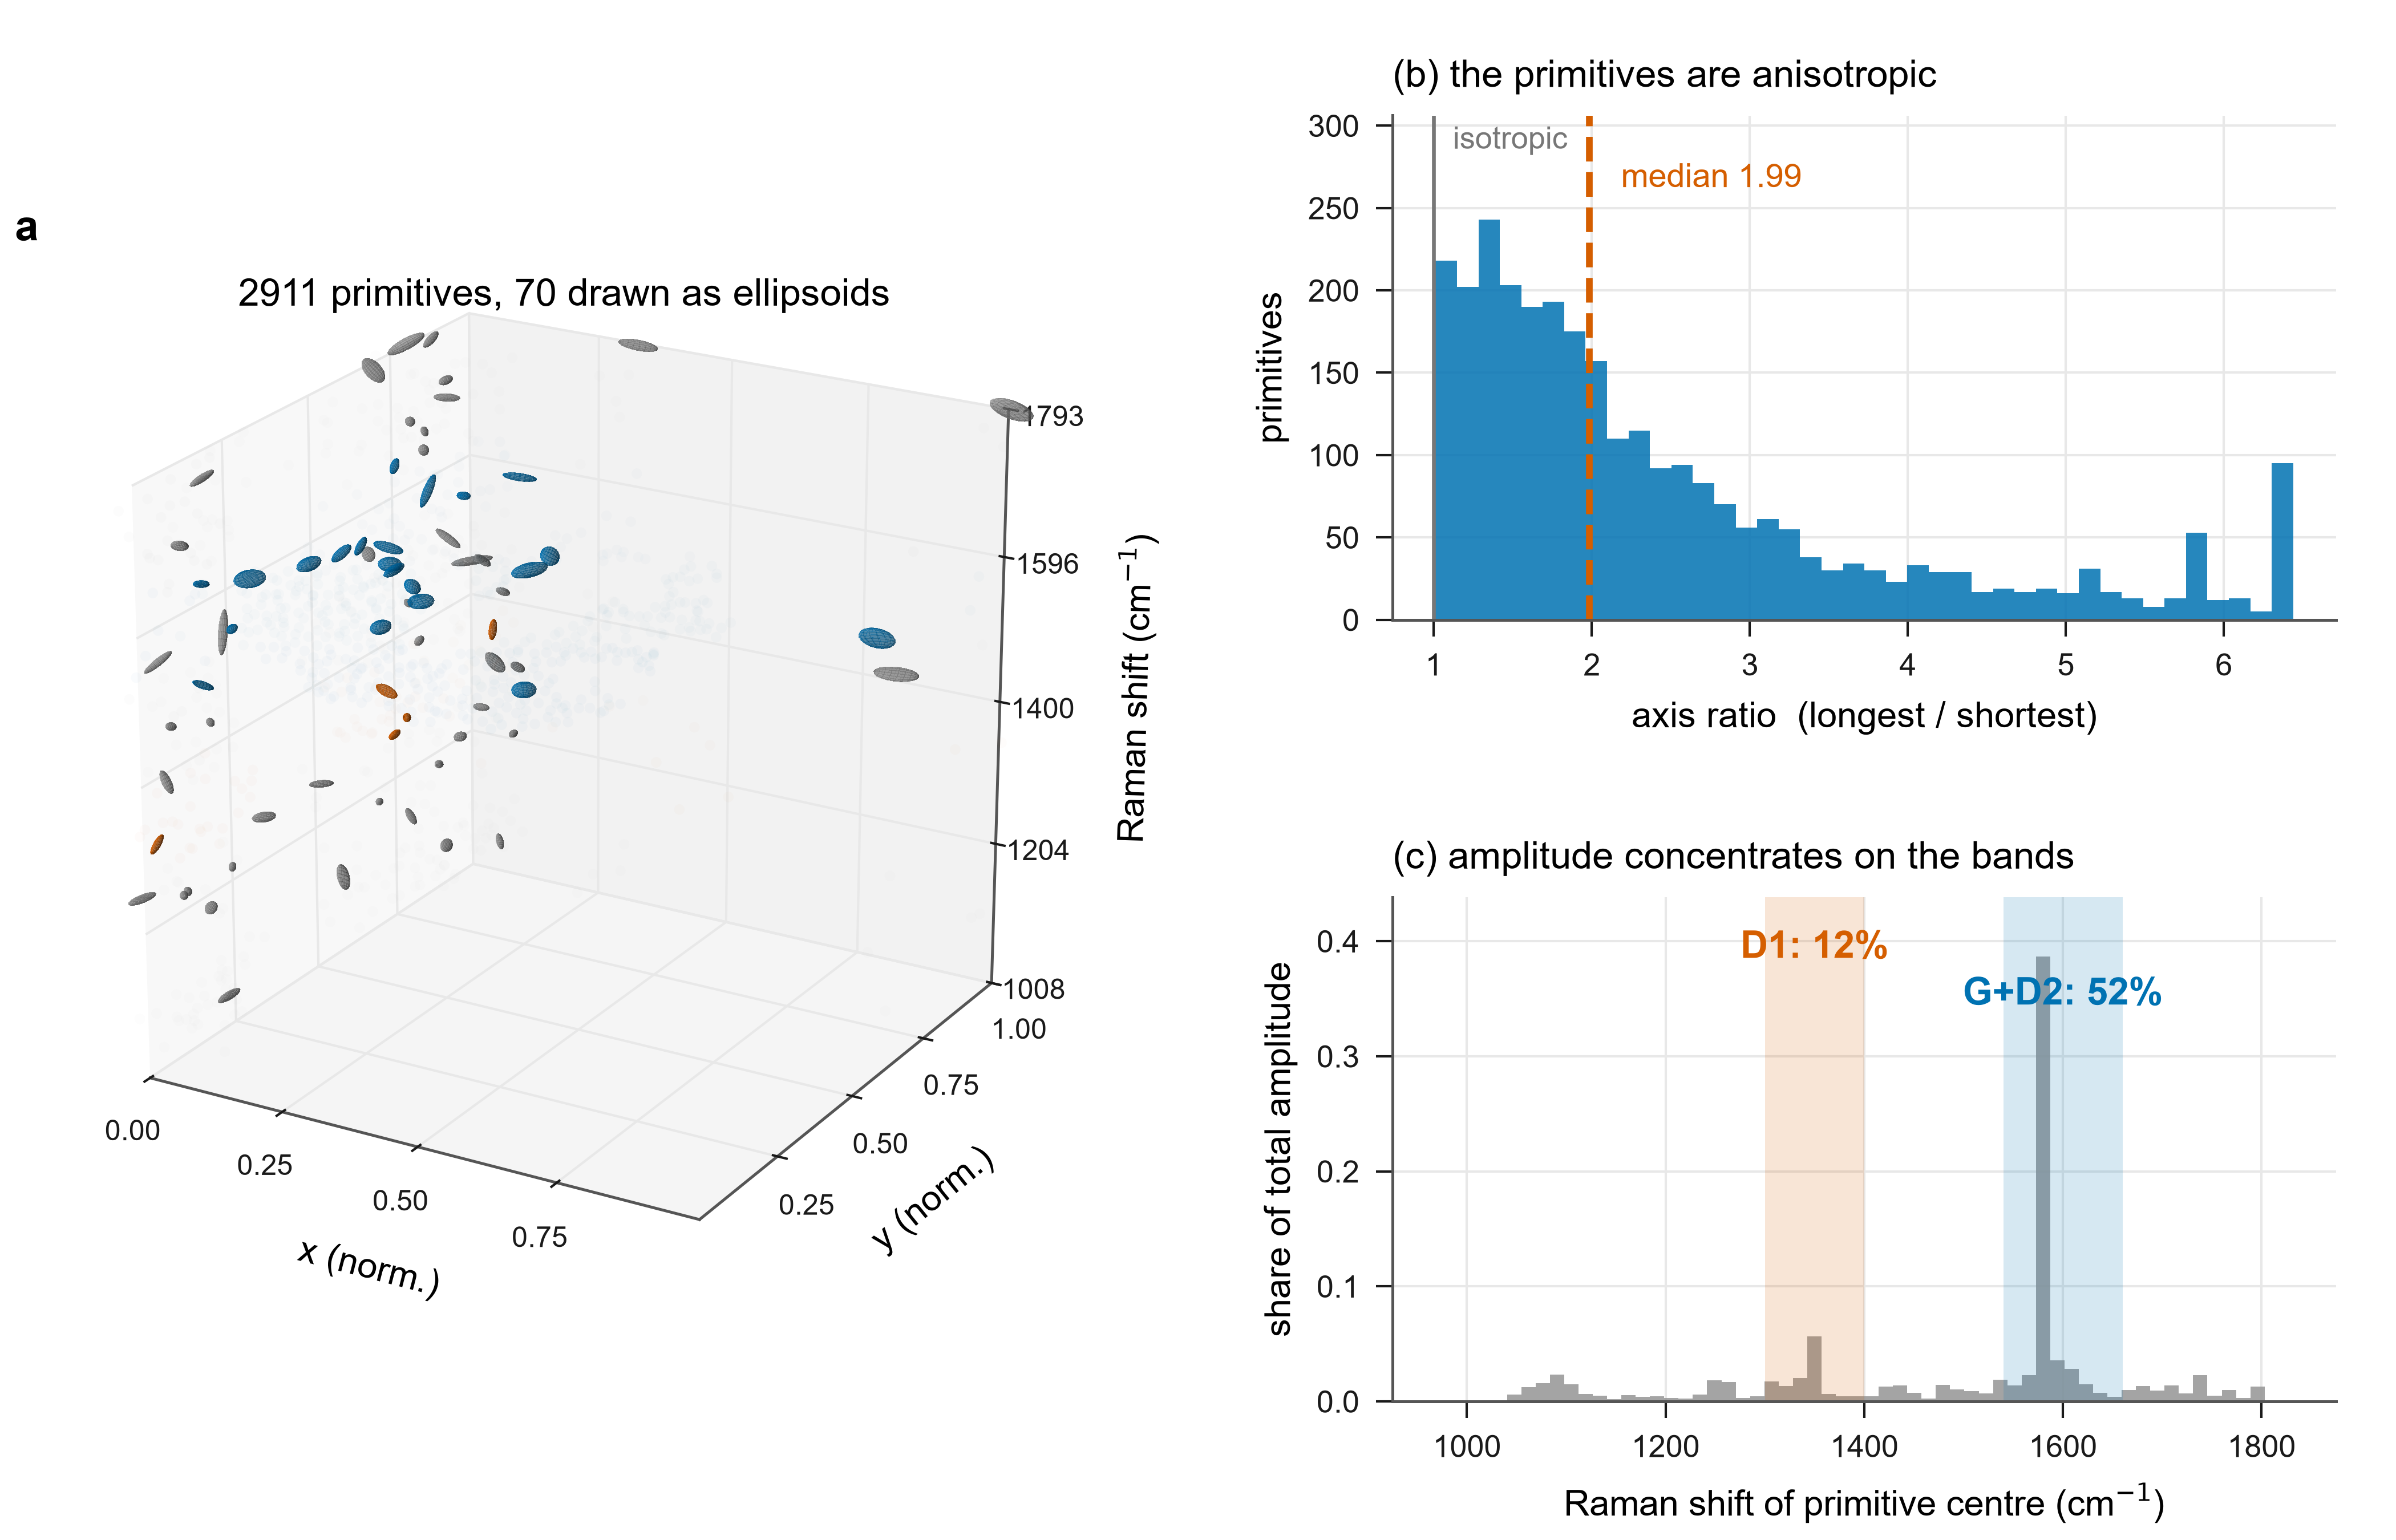
\includegraphics[width=\linewidth]{splat_acq-0042_ellipsoids}
\caption{Fitted primitives for acq-0042.}
\end{figure}

\clearpage
\begin{figure}[h]\centering
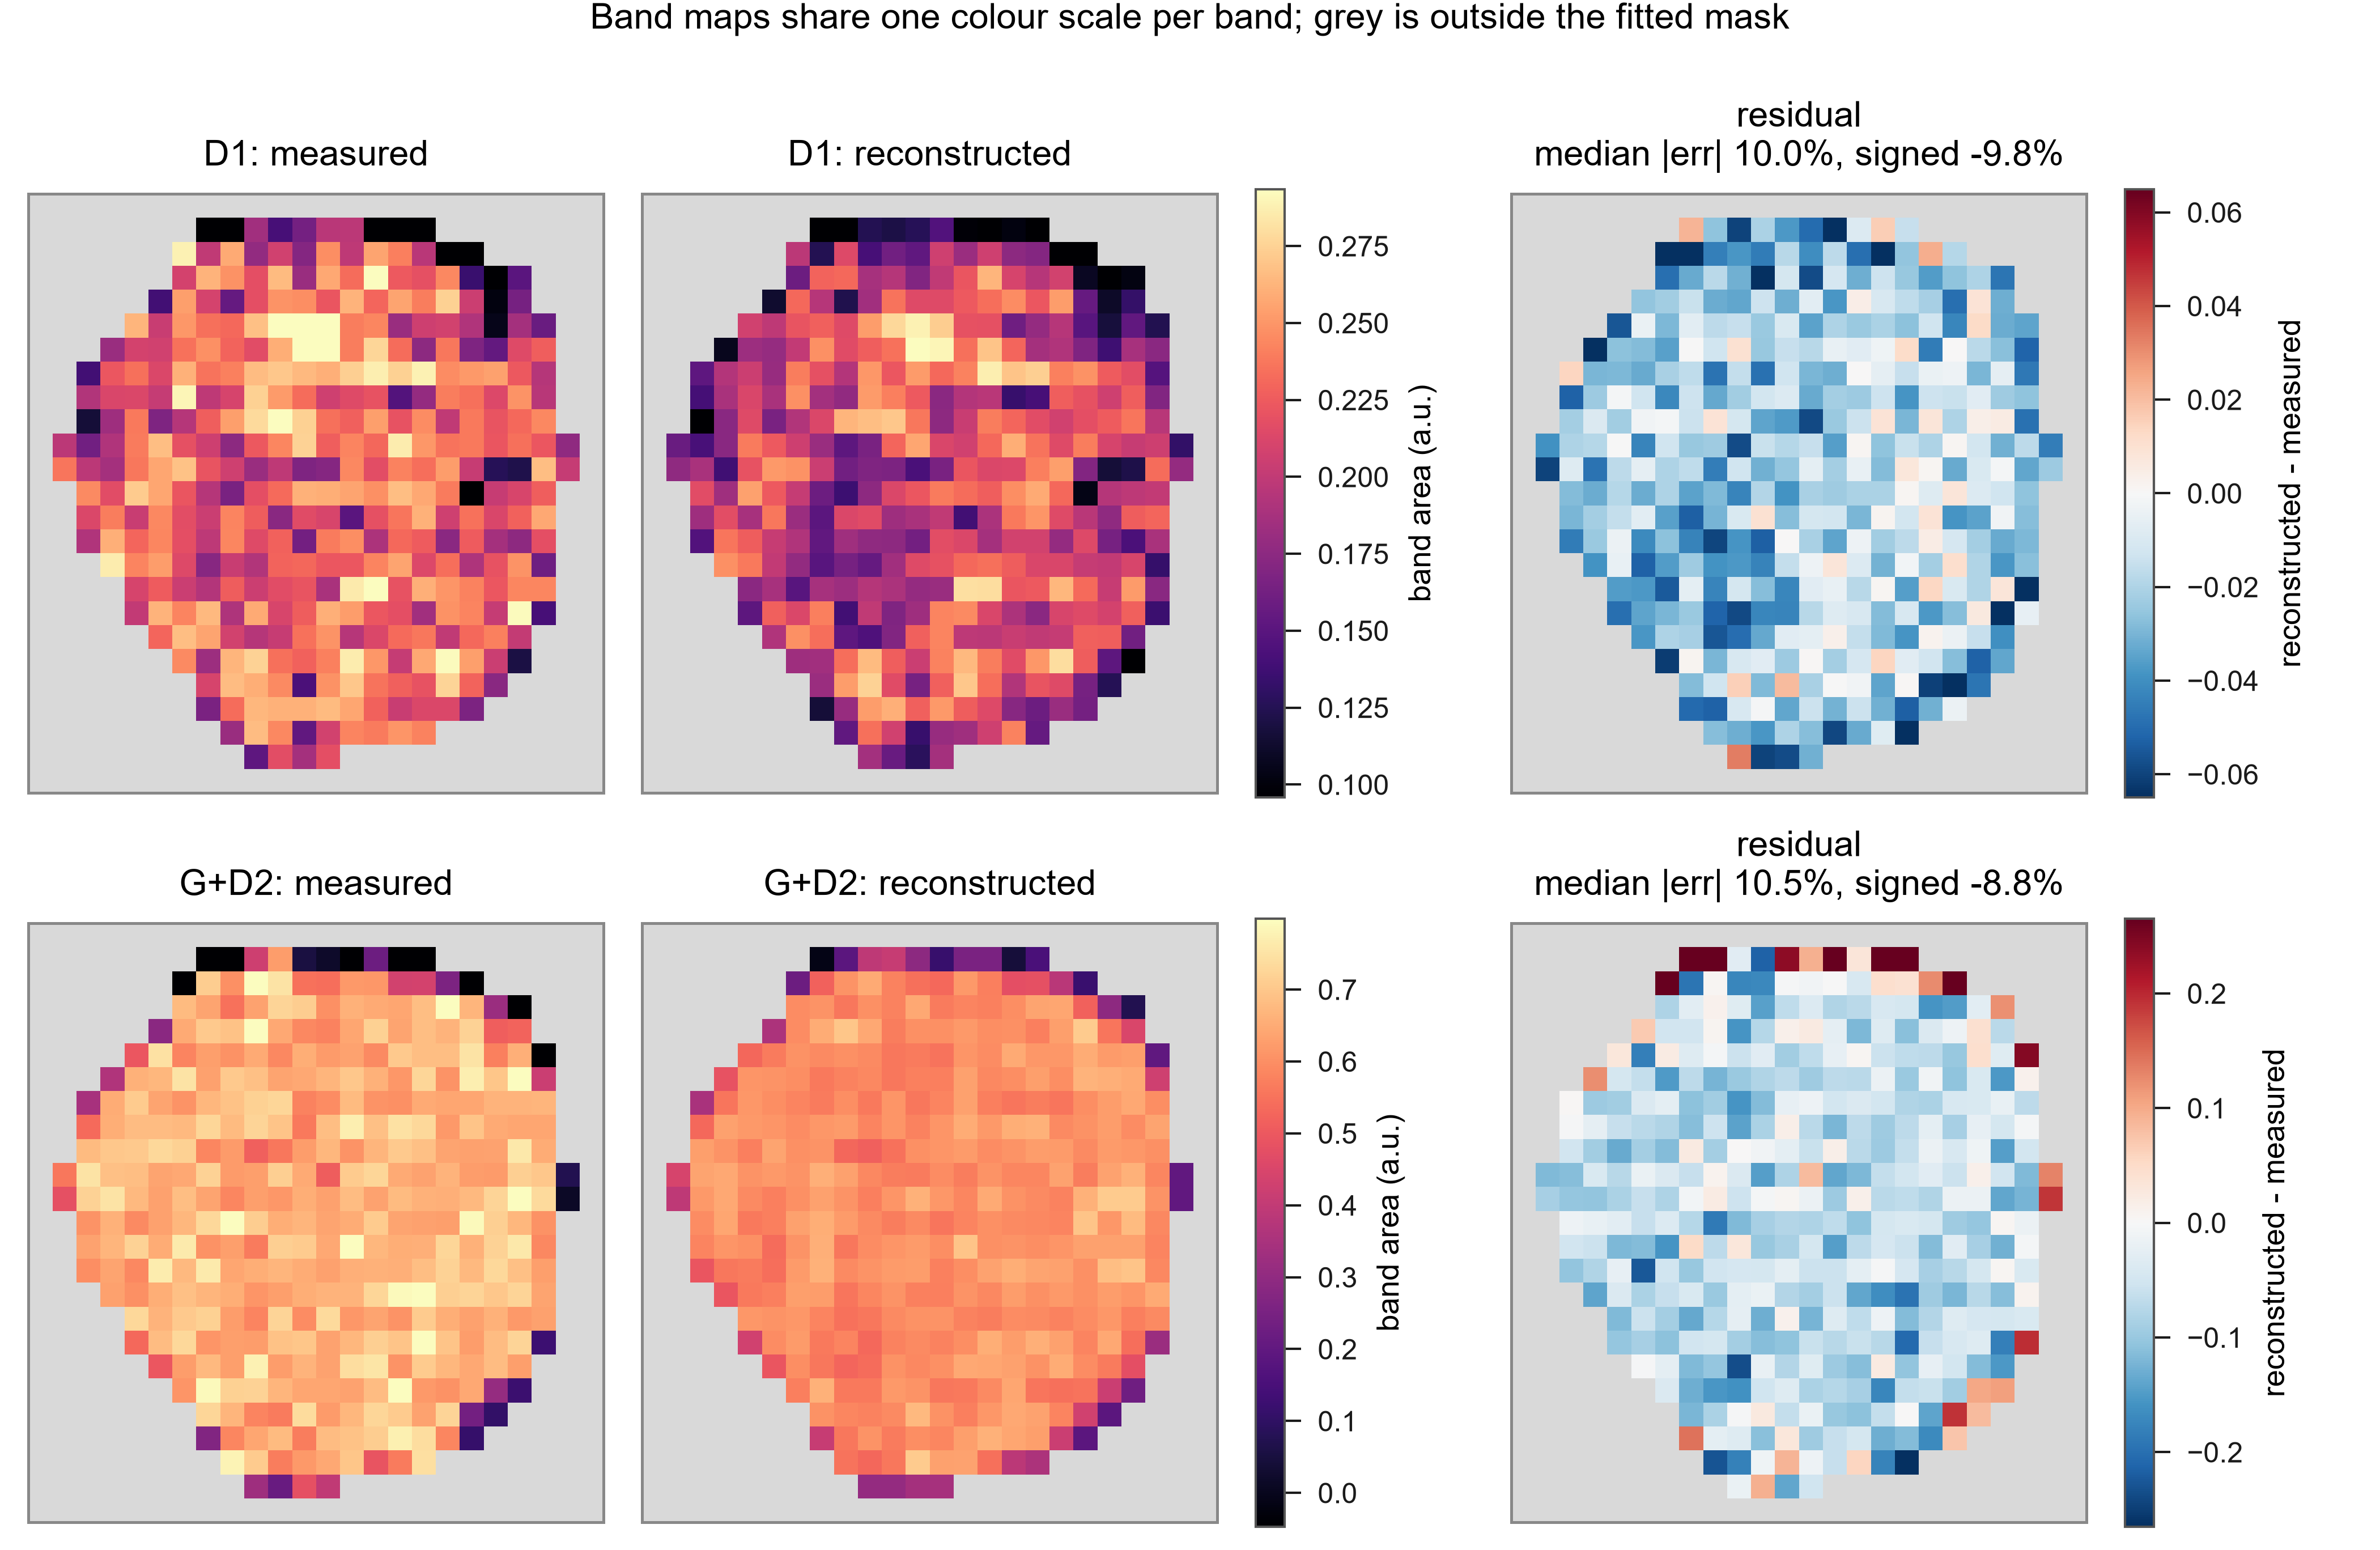
\includegraphics[width=\linewidth]{splat_acq-0055_bands}
\caption{Band maps for acq-0055, as Fig.~\ref{fig:si-bands-first}. This is the
smallest fitted map and the one whose held-out residual sits furthest below its
own noise floor.}
\end{figure}

\begin{figure}[h]\centering
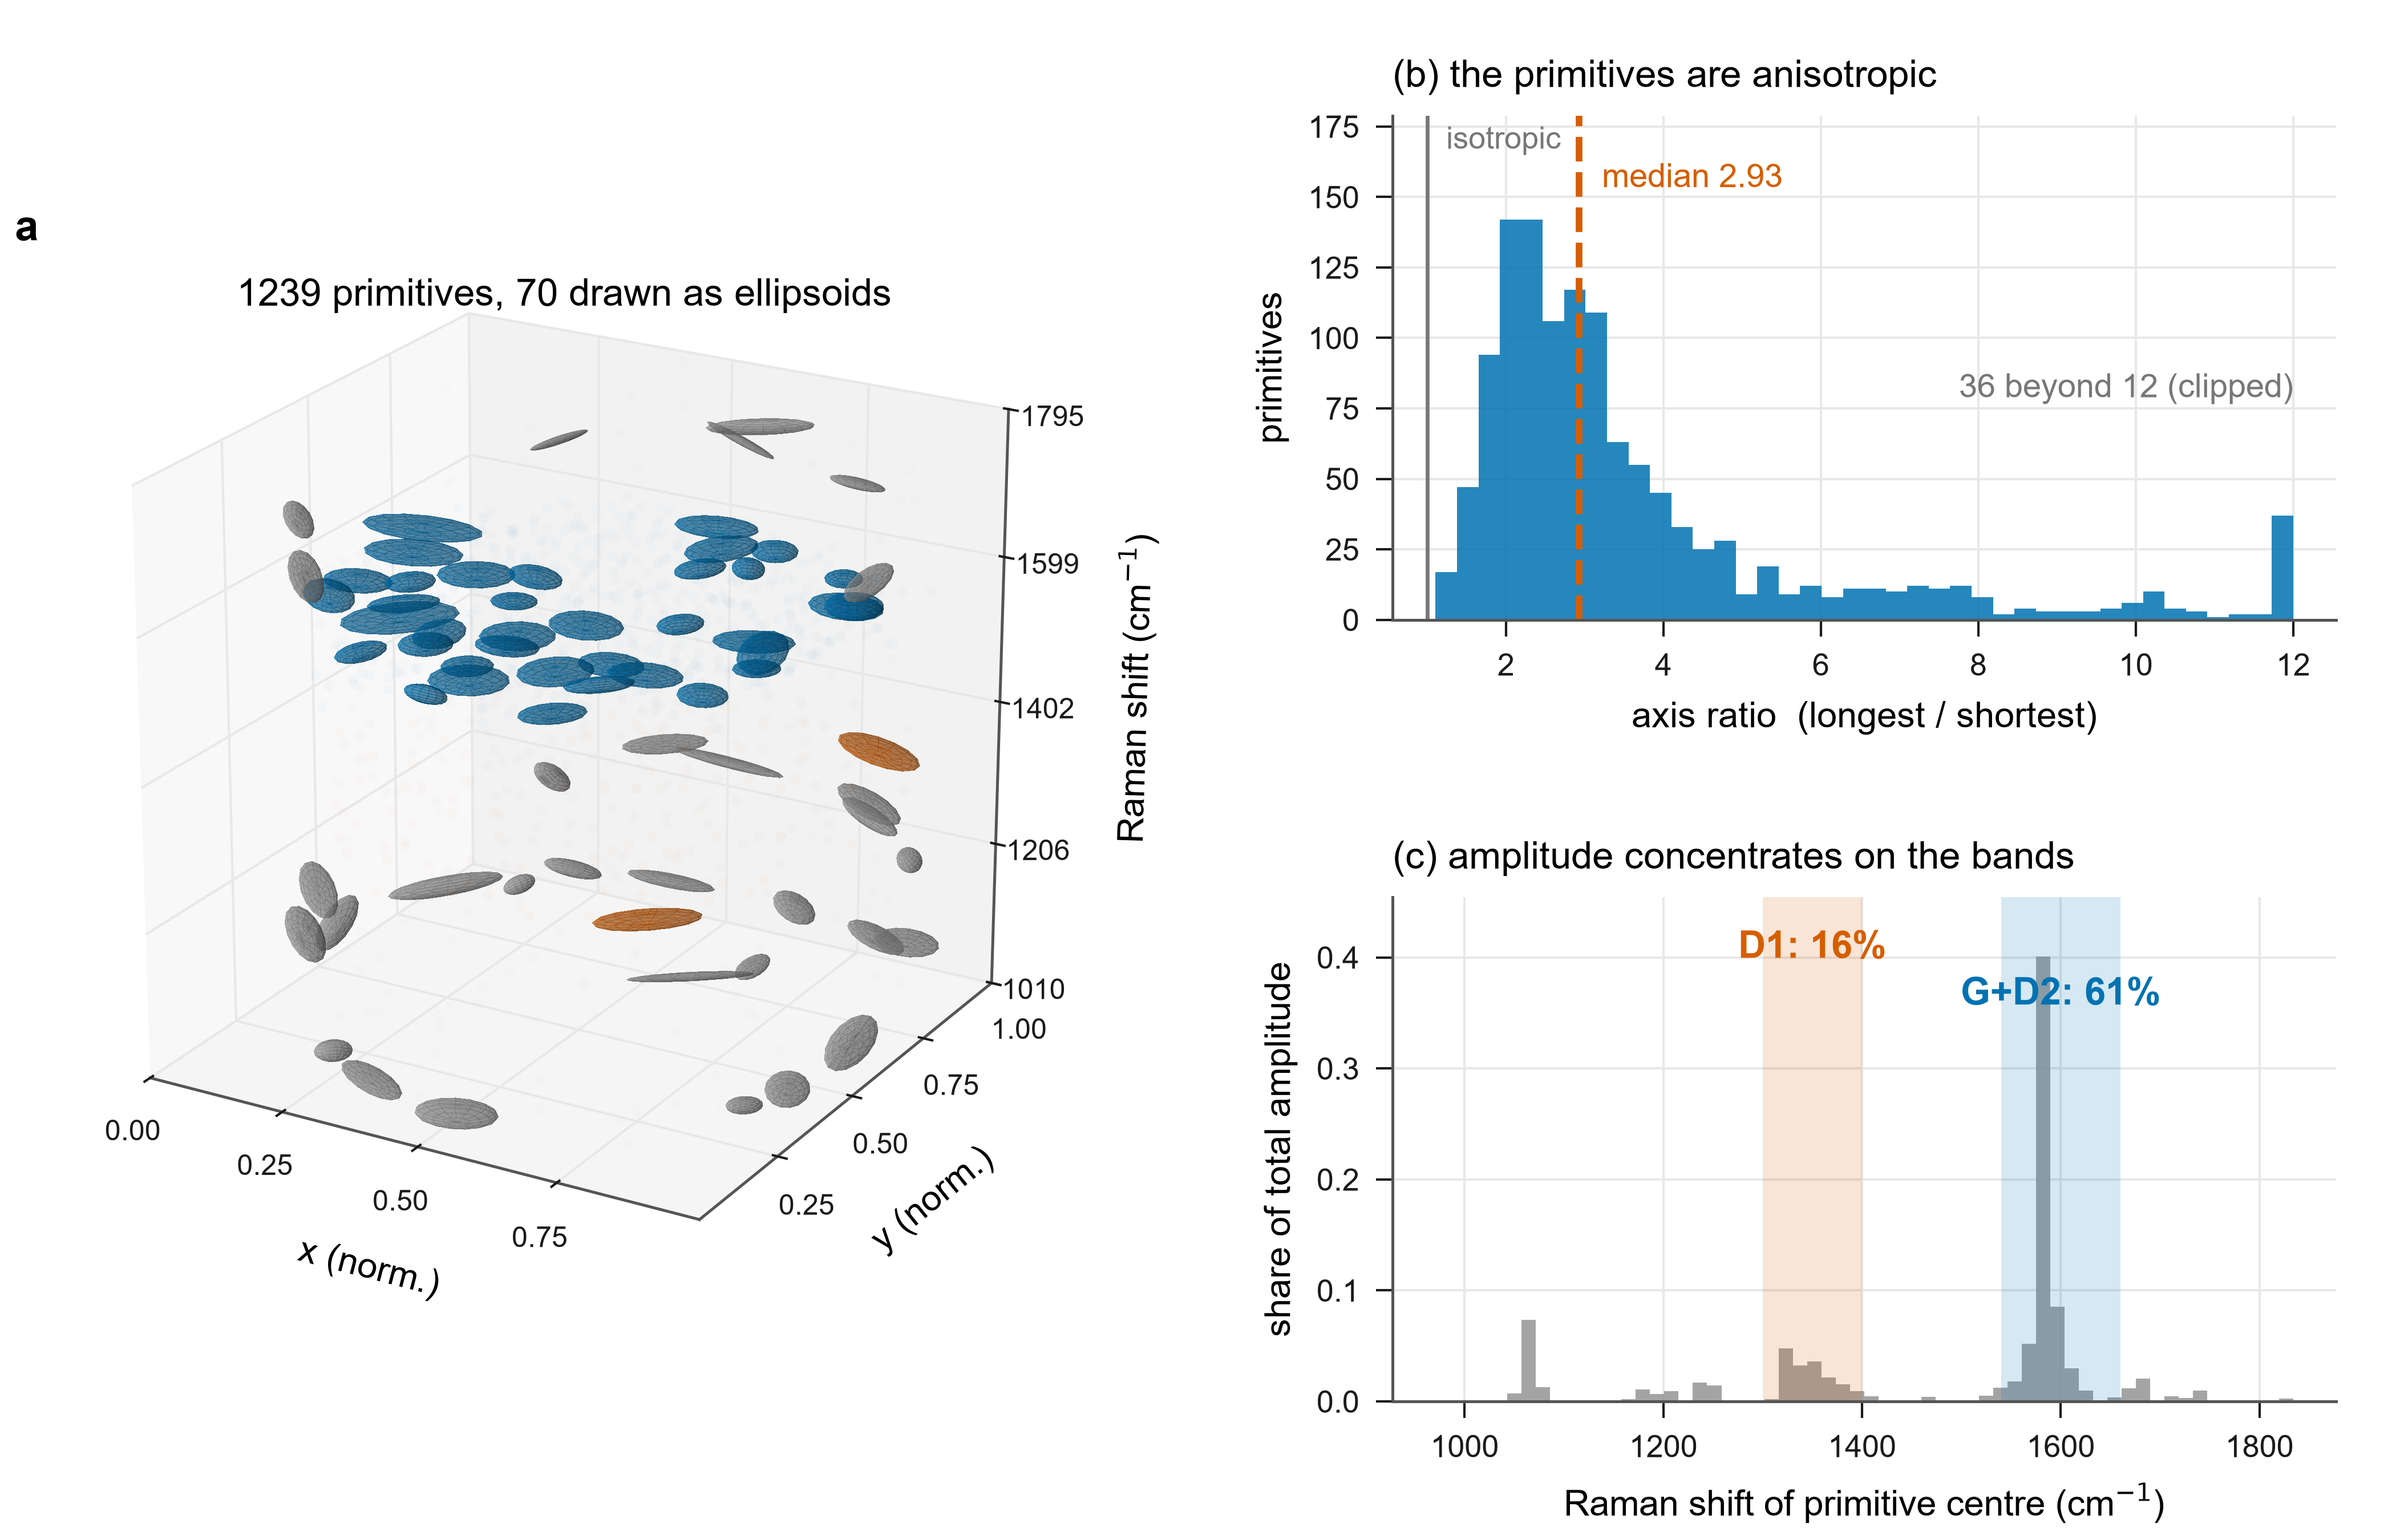
\includegraphics[width=\linewidth]{splat_acq-0055_ellipsoids}
\caption{Fitted primitives for acq-0055.}
\end{figure}

\clearpage
\section{Denoising benchmark, full table}

The benchmark contaminates every masked spectrum of the highest
contrast-to-noise map, \MLDenoiseMap, with additive Gaussian noise at
\num{1.5} times that map's own noise level, and scores \MLDenoiseN{} of them
against the uncontaminated original. Significance is a two-sided Wilcoxon
signed-rank test against \MLRefFilter, the best Savitzky-Golay filter, with
Benjamini-Hochberg correction across all method and metric pairs.

\begin{table}[h]\centering
\caption{Denoising benchmark. Lower is better throughout.}
\label{tab:si-denoise}
\small
\IfFileExists{tables/ml_denoise_tex.tex}
  {\begin{tabular}{lrrr}
\toprule
method & MSE & SAD & SID \\
\midrule
input (noisy) & 1.84e-08 & 0.0446 & 0.1340 \\
SG(2,5) & 6.71e-08 & 0.0630 & 0.1529 \\
SG(3,9) & 1.97e-07 & 0.0943 & 0.2837 \\
SG(3,15) & 6.3e-07 & 0.2001 & 0.8262 \\
SG(4,15) & 2.9e-07 & 0.1144 & 0.4155 \\
SG(3,21) & 9.58e-07 & 0.2862 & 1.1058 \\
SG(5,25) & 7.01e-07 & 0.2214 & 0.8947 \\
PCA (rank 217) & 1.59e-08 & 0.0415 & 0.1127 \\
S3DGS (ours) & 7.52e-07 & 0.1908 & 0.6960 \\
\bottomrule
\end{tabular}
}{(table not built)}
\end{table}

\section{Classifier benchmark, full table}

All \MLNmodels{} classifiers, both tasks, with accuracy, balanced accuracy and
weighted $F_1$ on held-out maps, are released as
\code{tables/ml\_models.csv}. Splits are by map, never by spectrum, because
spectra from one map share a specimen, a focus, a calibration and a noise
realisation and are therefore not independent samples. Models whose cost is
quadratic or cubic in the training-set size are fitted on a capped subsample,
and the cap is recorded alongside the score in that table so that no comparison
is silently unequal.

\section{Preprocessing ablation}

The ablation of the main text runs over the \AblNmaps{} smallest maps in the
corpus by masked point count, with up to 900 in-mask spectra drawn from each,
under \AblNproto{} named preprocessing protocols. Both limits exist to keep
five full preprocessing chains affordable and neither is chosen with reference
to the result. The per-map values are released as part of the figure manifest.

\end{document}
